%%%%%%%%%%%%%%%%%%%%%%% file template.tex %%%%%%%%%%%%%%%%%%%%%%%%%
%
% This is a general template file for the LaTeX package SVJour3
% for Springer journals.          Springer Heidelberg 2010/09/16
%
% Copy it to a new file with a new name and use it as the basis
% for your article. Delete % signs as needed.
%
% This template includes a few options for different layouts and
% content for various journals. Please consult a previous issue of
% your journal as needed.
%
%%%%%%%%%%%%%%%%%%%%%%%%%%%%%%%%%%%%%%%%%%%%%%%%%%%%%%%%%%%%%%%%%%%
%\begin{filecontents*}{example.eps}
%gsave
%newpath
%  20 20 moveto
%  20 220 lineto
%  220 220 lineto
%  220 20 lineto
%closepath
%2 setlinewidth
%gsave
%  .4 setgray fill
%grestore
%stroke
%grestore
%\end{filecontents*}
%
%\RequirePackage{fix-cm}
%
%\documentclass{svjour3}                     % onecolumn (standard format)
%\documentclass[smallcondensed]{svjour3}     % onecolumn (ditto)
\documentclass[smallextended,final]{svjour3}       % onecolumn (second format)
%\documentclass[twocolumn]{svjour3}          % twocolumn
%
\smartqed  % flush right qed marks, e.g. at end of proof
%
\usepackage[ruled,vlined,nofillcomment]{algorithm2e}
\usepackage{times}
\usepackage{graphicx}
\usepackage{verbatim}
\usepackage{setspace}
\usepackage{subfigure}
\usepackage{amssymb}
\usepackage{amsmath}
\usepackage{xspace}

\SetKwFor{PROCEDURE}{procedure}{}{}
\SetKwFor{EVENT}{on event receive}{do}{}
\SetKwFor{REPEAT}{repeat}{times}{}
\SetArgSty{textrm}

\SetKw{INTEGER}{int}
\SetKw{AND}{and}
\SetKw{OR}{or}
\SetKw{NOT}{not}
\SetKw{SEND}{send}
\SetKw{RECV}{recv}
\SetKw{TO}{to}
\SetKw{FROM}{from}

\newcommand{\clive}{\textsc{Clive}\xspace}
\newcommand{\tman}{\textsc{t-man}\xspace}
\newcommand{\glive}{\textsc{Glive}\xspace}
\newcommand{\adam}{\textsc{adam2}\xspace}
\newcommand{\cyclon}{\textsc{Cyclon}\xspace}
\newcommand{\cloudcast}{\textsc{CloudCast}\xspace}
\newcommand{\kompics}{\textsc{kompics}\xspace}
\newcommand{\cool}{\textsc{coolstreaming}\xspace}
\newcommand{\cyclop}{\textsc{Cyclop}\xspace}
\newcommand{\cloudangel}{\textsc{CloudAngel}\xspace}
\newcommand{\cloudmedia}{\textsc{CloudMedia}\xspace}
\newcommand{\angelcast}{\textsc{AngelCast}\xspace}
\newcommand{\croupier}{\textsc{Croupier}\xspace}

\newcommand{\BlockDuration}{\delta_c}
\newcommand{\BlockSize}{s_c}
\newcommand{\UpSlots}[1]{\mathit{Up}(#1)}
\newcommand{\DownSlots}[1]{\mathit{Down}(#1)}
\newcommand{\MaxMissing}{P_{\mathit{loss}}}
\newcommand{\tdelay}{T_{\mathit{delay}}}
\newcommand{\tlife}{T_{\mathit{life}}}
\newcommand{\tlcw}{T_{\mathit{lcw}}}
\newcommand{\rtt}{T_{\mathit{rtt}}}
\newcommand{\tround}{T_{\mathit{round}}}
\newcommand{\tlatency}{T_{\mathit{latency}}}
\newcommand{\Cah}{C_{\mathit{ah}}}
\newcommand{\Cvm}{C_{\mathit{vm}}}
\newcommand{\Cph}{C_{\mathit{ph}}}
\newcommand{\Cstorage}{C_{\mathit{storage}}}
\newcommand{\Creq}{C_{\mathit{req}}}
\newcommand{\Ctransfer}{C_{\mathit{chunk}}}
\newcommand{\Root}{{\mathit{root}}}
\newcommand{\DT}{{\mathit{DT}}}
\newcommand{\Depth}{{\mathit{depth}}}
\newcommand{\AH}{{\mathcal{AH}}}
\newcommand{\Nexp}{N_{\mathit{exp}}}
\newcommand{\Ntree}{N_{\mathit{tree}}}
\newcommand{\Nswarm}{N_{\mathit{swarm}}}

\newcommand{\Min}{\fontvar{min}}
\newcommand{\Slots}{\fontvar{slots}}

\newcommand{\fontproc}[1]{\texttt{\small #1}}
\newcommand{\fontvar}[1]{\mathit{#1}}
\newcommand{\Density}{\textsc{Density}\xspace}
\newcommand{\treesize}{\fontproc{size}}
\newcommand{\treesizerec}{\fontproc{recSize}}
\newcommand{\MIN}{\fontproc{min}}
\newcommand{\Random}{\fontproc{random}}
\newcommand{\round}{\fontproc{round}}
\newcommand{\init}{\fontproc{init}}
\newcommand{\poll}{\fontproc{poll}}
\newcommand{\MergeView}{\fontproc{mergeView}}
\newcommand{\updateage}{\fontproc{updateAge}}
\newcommand{\selectoldest}{\fontproc{selectOldest}}
\newcommand{\remove}{\fontproc{remove}}
\newcommand{\add}{\fontproc{add}}
\newcommand{\randomsubset}{\fontproc{randomSubset}}
\newcommand{\request}{\fontproc{REQ}}
\newcommand{\reply}{\fontproc{RES}}
\newcommand{\maxslot}{\fontproc{maxSlot}}
\newcommand{\slot}{\fontproc{slot}}
\newcommand{\sv}{\fontproc{SV}}
\newcommand{\subview}{\fontproc{subview}}

\newcommand{\fakeparagraph}[1]{\vspace{8pt}\noindent\textbf{#1}}

% \usepackage{mathptmx}      % use Times fonts if available on your TeX system
%
\begin{document}

\title{CLive: Hybrid P2P-Cloud Live Streaming}
\titlerunning{CLive: Hybrid P2P-Cloud Live Streaming}        % if too long for running head

\author{Amir H. Payberah \and Hanna Kavalionak \and Alberto Montresor \and Seif Haridi}

\institute{Amir H. Payberah and Seif Haridi \at
SICS, Isafjordsgatan 22, Box 1263, SE-164 29 Kista, Sweden \\
\email{\{amir,seif\}@sics.se}   \\
Hanna Kavalionak and Alberto Montresor \at
Dept. of Information Engineering and Computer Science, University of Trento, Italy\\
\email{\{hanna.kavalionak,alberto.montresor\}@unitn.it}        %  \\
}

\date{Received: date / Accepted: date}

\maketitle

\begin{abstract}
Peer-to-peer (P2P) overlays have lowered the barrier to stream live events
over the Internet, and have thus revolutionized the media streaming
technology. However, satisfying soft real-time constraints on the delay
between the generation of the stream and its actual delivery to users is still
a challenging problem. Bottlenecks in the available upload bandwidth, both at
the media source and inside the overlay network, may limit the quality of
service (QoS) experienced by users. A potential solution for this problem is
to \emph{assist} the P2P streaming network by a cloud computing infrastructure
to guarantee a minimum level of QoS. In such approach, rented cloud resources
({\em helpers}) are added on demand to the overlay to increase the amount of
total available bandwidth and the probability of receiving the video on time.
Hence, the problem to be solved becomes minimizing the economical cost,
provided that a set of constraints on QoS is satisfied. The main contribution
of this paper is \clive, a cloud-assisted P2P live streaming system that
demonstrates the feasibility of these ideas. \clive estimates the available
capacity in the system through a gossip-based aggregation protocol and
provisions the required resources from the cloud to guarantee a given level of
QoS at low cost. We perform extensive simulations and evaluate \clive using
large-scale experiments under dynamic realistic settings.
\keywords{P2P Live Streaming \and Gossip-based Algorithm \and P2P-Cloud Overlay Network}
\end{abstract}

\section{Introduction} \label{sec:introduction}

Nowadays, video streaming of live events is one of the hottest application of the peer-to-peer (P2P) paradigm. Unlike many other P2P services that failed
to go beyond the lab of an university, the strong academic push towards
this technology~\cite{qoe,gossip++,glive,gradientv,sepidar} has been quickly paired by large investments from commercial companies~\cite{sopcast,roverso2012smoothcache,pplive}.

The main challenge of a decentralized video streaming service is to strike a good balance between \emph{playback continuity} and \emph{playback
delay}. These two properties, which together with the video resolution define the quality of service (QoS) of a video streaming service, are linked by a trade-off:
it is possible to increase the playback continuity, i.e., to obtain a smooth
media playback, by adopting larg\-er stream buffers, but at the expense
of delay. On the other hand, improving playback delay requires that no
bottlenecks are present in either the upload bandwidth of the media source and
the aggregated upload bandwidth of all nodes in the \emph{swarm}, i.e., the
nodes forming the P2P streaming overlay~\cite{CloudAngel}.


Increasing the bandwidth at the media source may be difficult, as these systems
are exactly designed to cope with situations where the source is an off-the-shelf machine provided with a standard Internet connection. Even when
possible, bottlenecks in the swarm have proven to be much more
disruptive~\cite{Kumar:MDT}. The approach proposed in this paper to solve
this issue is to add auxiliary \emph{helpers} aimed at accelerating the content 
propagation.  A helper could
be an \emph{active} computational node that participates in the streaming
protocol, or a \emph{passive} storage service that just provides
content on demand. The helpers increase the total upload bandwidth available
in the system, thus, potentially reducing the playback delay. Both types of
helpers could be rented on demand from a cloud provider, e.g., Amazon AWS, with different prices. 

This P2P-cloud hybrid approach is nothing
new: a number of P2P content distribution systems~\cite{CloudAngel,cloudcast,Sripanidkulchai,sripanidkulchai2004analysis} have already been pursued under the name of \emph{cloud-assisted} P2P computing.
What is novel here is the combination of two different types of helpers, active and passive, that are carefully selected and provisioned
with respect to the dynamic behavior of the users. If not enough
helpers are present, it is impossible to achieve the desired level of
QoS. On the other hand, renting helpers is costly, and their number should be
minimized.

The contribution of this paper is to model this problem as an optimization one,
where the constraints are given by the desired QoS level with respect to playback continuity and playback delay, while the objective
function is to minimize the total economic cost incurred in renting resources from the cloud. We provide \clive a decentralized on-line system that is adaptive to dynamic networks.

\clive guarantees the QoS at nodes by including a passive helper (PH), e.g., cloud storage, whose task is to provide a last resort for nodes that have not been able to obtain their video chunks through the swarm. Hence, if a node can not receive the required video chunks on time from other nodes in the swarm, it downloads them from the PH. We assume that the media source pushes the new generated video chunks to the PH, so it always contains the latest chunks. However, any interaction with the PH is associated with a cost, and since our objective function is to minimize the cost, we need to reduce the communication with the PH as much as possible.

A solution to reduce the PH cost is to take advantage of active helpers (AH), which are added/removed dynamically on demand. AHs are high upload bandwidth nodes that actively participate in the swarm. The more AHs are added to the system, the more chance nodes have to receive chunks from the swarm, thus, they refer to PH less often, and it consequently reduces the cost of communication with PH. However, the AHs are also costly themselves, therefore, a delicate balance between the amount of video chunks obtained from the PH and the number of AHs in the system must be found. In other word, AHs should be added to the system such that their cost does not exceed the reduced cost caused by less communication with the PH.

To solve this problem, \clive exploits a module called \clive manager (CM) that uses a gossip-based technique to monitor the state of the swarm, estimate the available upload bandwidth in the system, and based on that computes the proper number of required AHs. To summarized, \clive uses PH to guarantee the QoS, i.e., all nodes receive the video chunks on time, and it adds/removes AHs just to reduce the total cost (if possible).

To demonstrate the feasibility of \clive, we performed extensive simulations
and evaluate our system using large-scale experiments under dynamic realistic
settings. We show that we can save up to $45\%$ of the cost by choosing the
right number of active helpers compared to only using a passive helper to
guarantee the predefined QoS.

\section{System model and problem definition} \label{sec:problem}

We consider a network consisting of a dynamic collection of \emph{nodes} that
communicate through message exchanges. Nodes could be \emph{peers}, i.e., edge
computers belonging to users watching the video stream, \emph{helpers}, i.e.,
computational and storage resources rented from a cloud, and the
\emph{media source} (\emph{source} for short) that generates the video
stream and starts its dissemination towards peers.

Each peer is uniquely identified by an ID, e.g., composed by IP address and
port, required to communicate with it. We use the term \emph{swarm} to refer
to the collection of all peers. The swarm forms an \emph{overlay network},
meaning that each peer connects to a subset of peers in the swarm (called
\emph{neighbors}). The swarm is highly dynamic: new peers may join at any
time, and existing peers may voluntarily leave or crash. Byzantine behavior is
not considered in this work. We assume that peers are approximately synchronized; this is a reasonable
assumption, given that some cloud services, like Amazon AWS, are already
synchronized and sometimes require the client machines to be synchronized as
well.

The goal of \clive peers is to play the video with predefined \emph{playback delay} (the time between the generation of the video and its visualization at the peer) and \emph{playback continuity} (the percentage of chunks that are correctly streamed to users). A trivial solution to improve the users' viewing experience is to increase the buffering time at end points. The more buffering time users have, the higher is the playback continuity. On the other hand, a large buffering time increases the playback delay, which is not acceptable. Hence, the buffering time should be chosen such that it is long enough to compensate for the late received chunks, but not too long to disrupt the playback delay. Nevertheless, even if the buffering time is chosen properly, it still requires that no bottleneck exists in the swarm upload bandwidth, otherwise again users would not be able to download chunks on time. Since the high buffering time is not a suitable solution, and bottlenecks in the swarm upload bandwidth are very 
likely to happen~\cite{Kumar:MDT}, we use helpers, rented from the cloud, to guarantee playback continuity at users with a short playback delay.


There are two types of helpers: (i) \emph{active helper} (AH), an
autonomous virtual machine composed of one or more computing cores, volatile
memory and permanent storage, e.g., Amazon EC2, and (ii) \emph{passive
helper} (PH), a simple storage service that can be used to store and
retrieve arbitrary pieces of data, e.g., Amazon S3. We assume that
customers of the cloud service are required to pay for computing time and
bandwidth in the case of AHs, and for storage space, bandwidth and the number
of interactions with the PH. This model follows the Amazon's
pricing model~\cite{amazonec2,amazons3}.

We assume the source generates a constant-rate bitstream and divides it into a
number of \emph{chunks}. A chunk $c$ is uniquely identified by the real time
$t(c)$ at which is generated. The generation time is used to play chunks in
the correct sequence, as they can be retrieved in any order, independently from
previous chunks that may or may not have been obtained yet.

Peers, helpers and the source are characterized by different bounds on the
amount of available download and upload bandwidth. A peer can create a bounded
number of download connections and accept a bounded number of upload
connections over which chunks are downloaded and uploaded. We define the
number of {\em download slots} and {\em upload slots} of a peer as the
largest number of download and upload connections that it can sustain, respectively. 
Thanks to the replication strategies between different data centers currently employed in
clouds~\cite{goel2006data}, we assume that PH has an unbounded number of
upload slots and can serve as many requests as it receives. Although the PH is logically one service, it could be implemented using  a geographically replicated service. We have performed preliminary experiments using Amazon Cloudfront that enabled us to serve chunks from different geographical locations.

To reach the \clive goal, i.e., high playback continuity and short playback delay, \clive is allowed to rent 
PH and/or AH resources from the cloud. 
We model our problem as an optimization one, where the objective function to be minimized is the total economic cost incurred from renting active helpers and passive helpers from the cloud, subject to the following QoS constraints:
\begin{enumerate}
\item the maximum playback delay should be less than or equal to $\tdelay$,
meaning that if a chunk $c$ is generated at time $t(c)$ at the source, no
peers will show it after time $t(c)+\tdelay$;
\item the maximum percentage of missing chunks should be less than or equal the predefined threshold.
\end{enumerate}

Finding the optimum answer, i.e., lowest cost, of this problem requires a complete and accurate knowledge of the system, which is impossible in a dynamic network, where peers join and fail continuously. Even in a static network, where there is no churn, the optimum solution depends on the overlay structure. However, constructing the swarm overlay is out of the scope of this paper. In Section~\ref{sec:cmmanager}, we present our heuristic to reduce the total cost as much as possible, and in Section~\ref{sec:evaluation}, we show that in a static and homogeneous network, where we have the accurate knowledge, we can achieve the minimum cost.

\begin{figure*}[t]
\centering
\subfigure[\scriptsize The baseline model.]{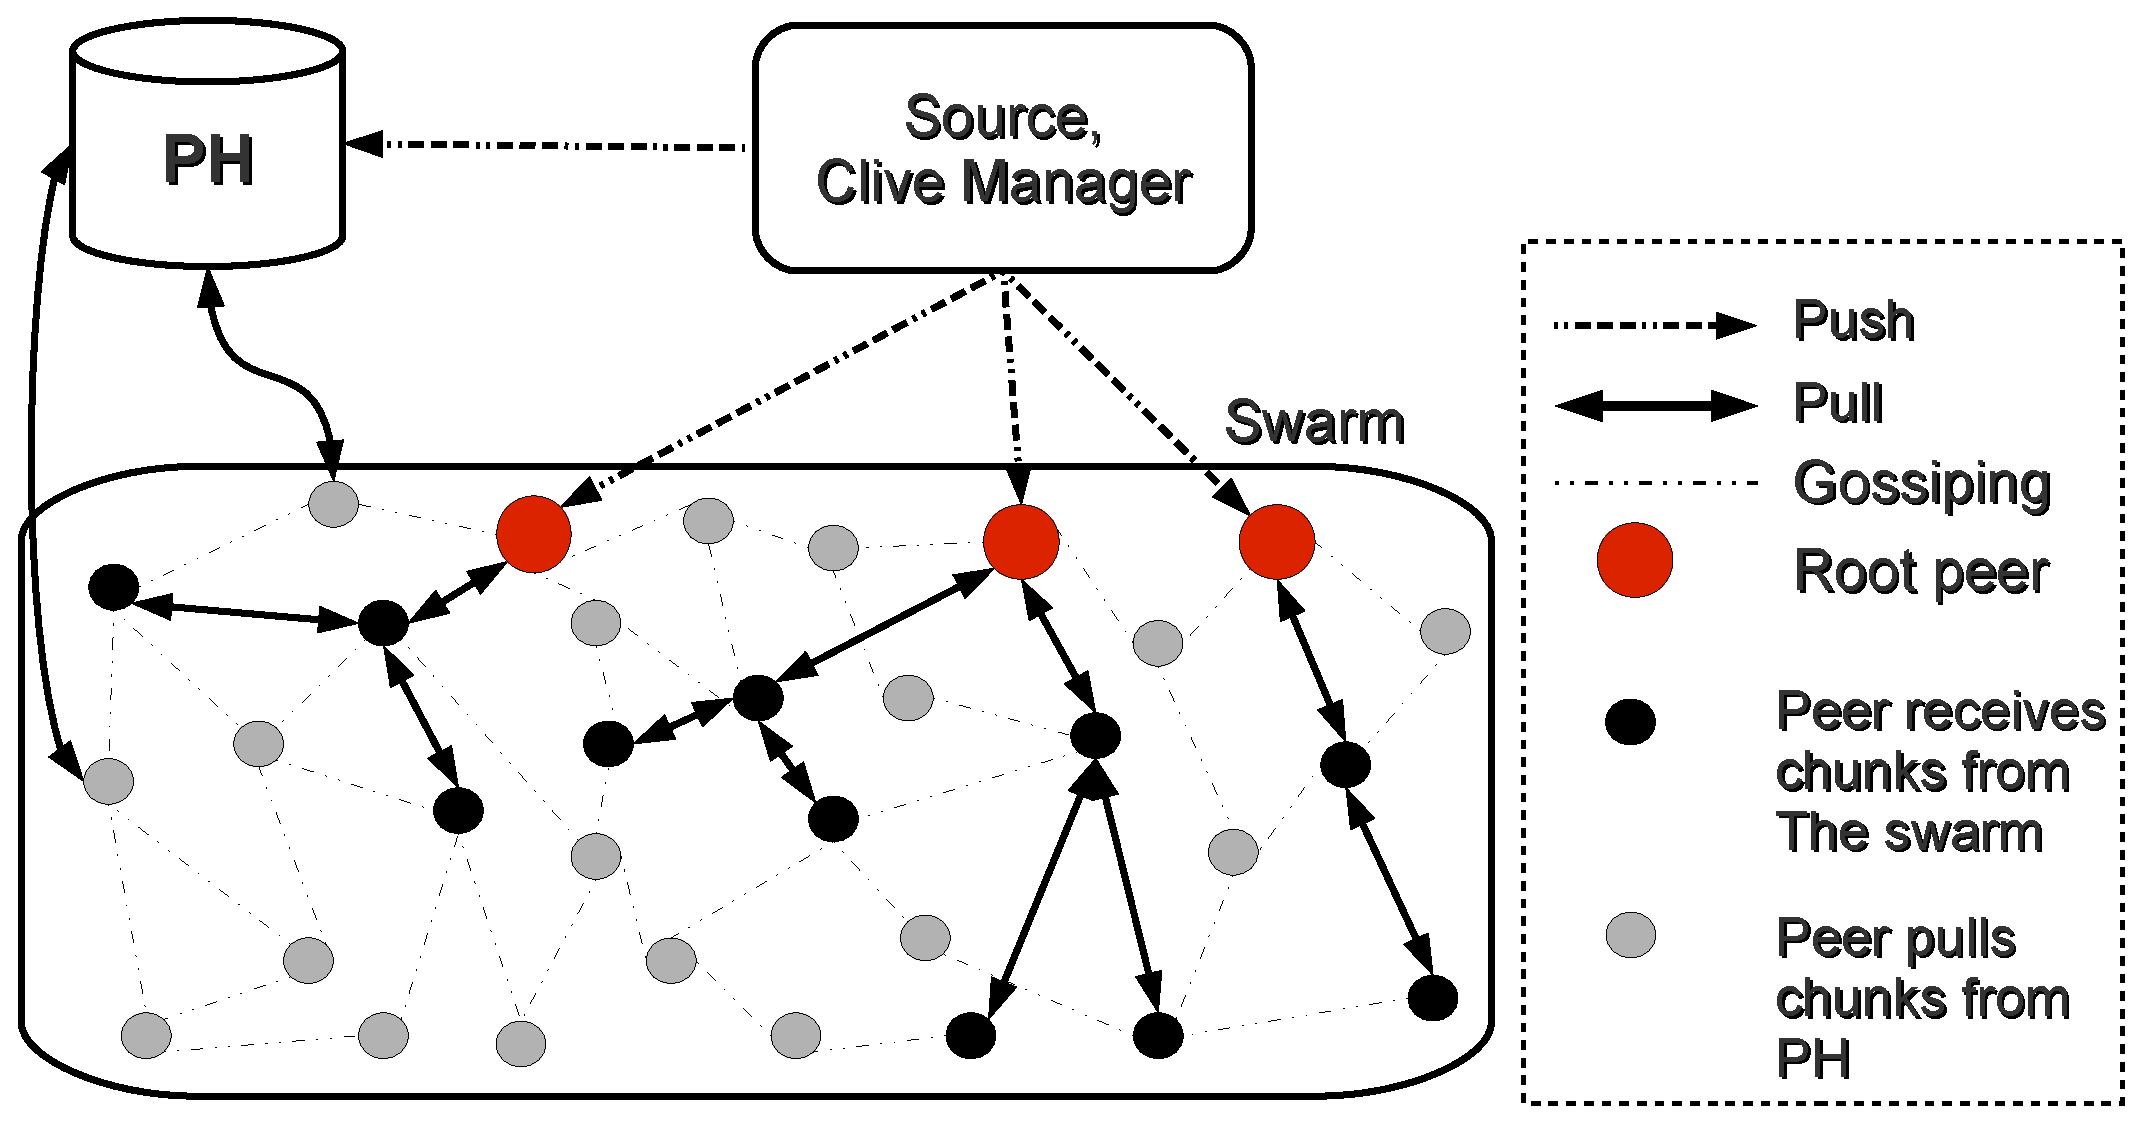
\includegraphics[angle=0, width=0.7\columnwidth]{base}\label{fig:arch1}}
\subfigure[\scriptsize The enhanced model.]{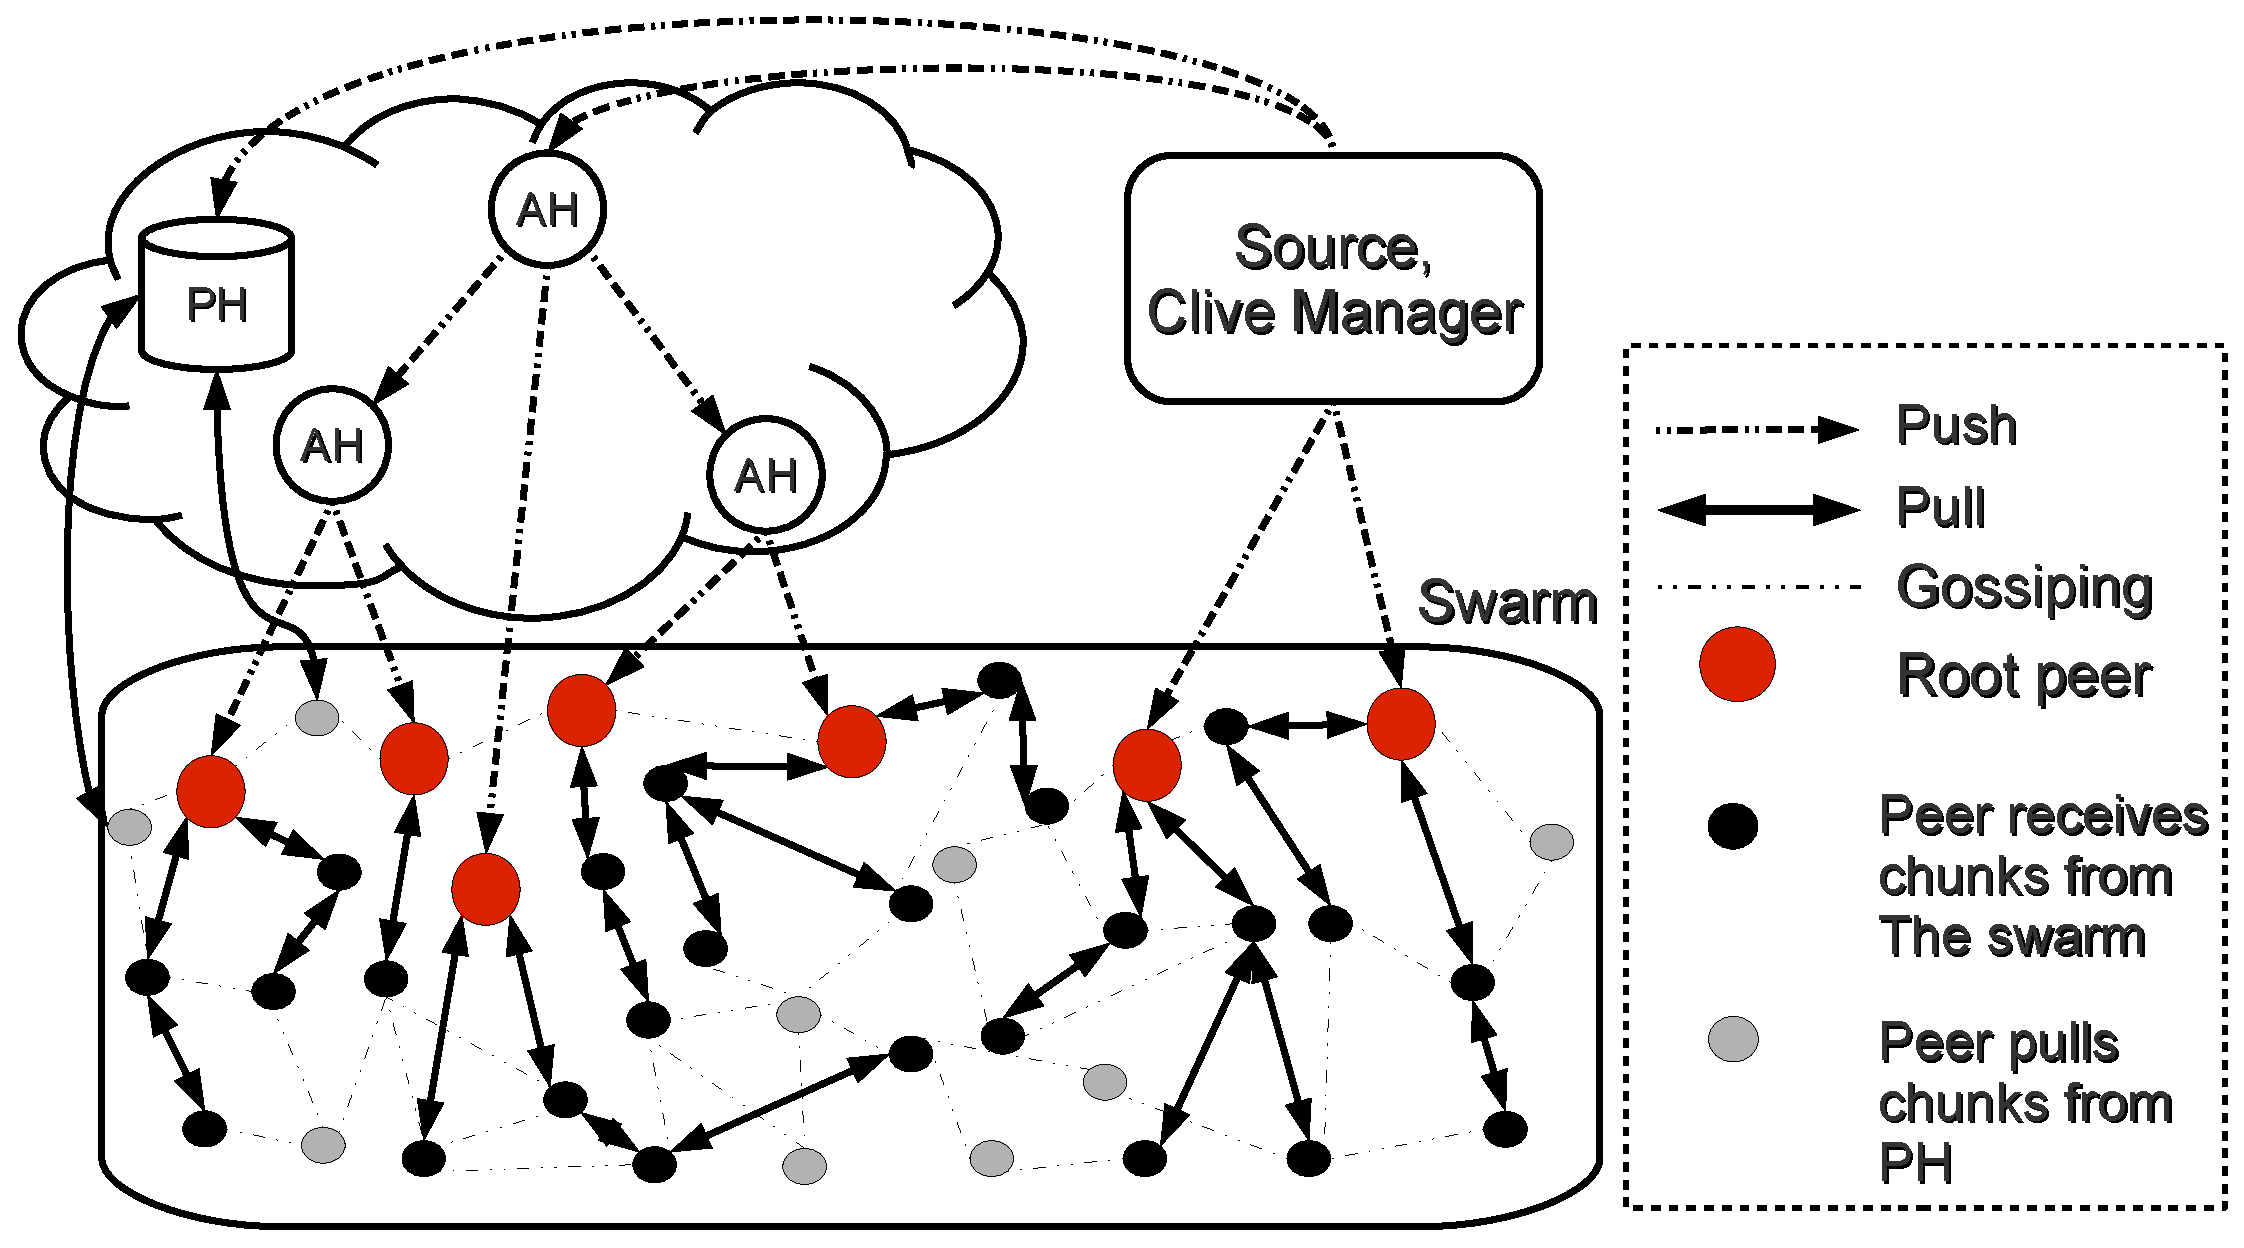
\includegraphics[angle=0, width=0.7\columnwidth]{enhanced}\label{fig:arch2}}
\caption{\small The system architecture}\label{fig:arch}
\end{figure*}


\section{System architecture} \label{sec:system}
We present two architectural models, illustrated
in Figures~\ref{fig:arch1} and~\ref{fig:arch2}. The \emph{baseline} model
(Figure~\ref{fig:arch1}) can be described as a P2P streaming protocol, where
peers revert to PH whenever a chunk cannot be retrieved from other peers on time. The
\emph{enhanced} model (Figure~\ref{fig:arch2}) builds upon the baseline, by
considering AHs and by providing a distributed mechanism to provision their
number and appropriately organizing them. 

The main idea behind these models is as follows: to overcome the bottleneck in the swarm upload bandwidth, we rent extra resources from a cloud provider. In the baseline solution, only one PH, i.e., storage, is rented from a cloud provider. In this model, the source pushes chunks to the PH in addition to the swarm. Hence, when a peer cannot receive a chunk of data from other peers in the swarm, it pulls that chunk from the PH. This model guarantees that all peers receive the whole chunks on time. The PH is on a cloud, and clearly we cannot get 100\% availability. However, we assume that the PH is always available in our system, because when the cloud fails, there is nothing we can do.

The baseline model could be costly, if the number of requests at the PH increases. A solution to reduce the PH load is to rent AHs in addition to the PH. AHs actively participate in data dissemination with other peers, and thus, reduce the PH usage. Given that the cost of AH and PH are different, we select the optimal number of AHs that produce the minimum total cost while delivering the desired QoS. 

To compute the number of AHs, we use a distributed aggregation protocol to estimate the available upload bandwidth in the system, as well as the number of peers that can receive chunks on time using the existing resources without the help of PH. Then, based on these estimations, \clive manager (CM) periodically adds/removes AHs to/from the system in rounds.

To prevent any noise and fluctuation in the number of AHs, only one AH is added/removed to/from the system in each round of the resource management, regardless of the total required AHs. Meanwhile AHs are added/removed, the peers can pull required chunks from the PH. Note that the lack of AHs in the system does not violate the QoS at peers, because although they help in data dissemination, their net effect is on the cost, and the QoS is guaranteed by the PH. When an AH joins the system, it just reduces the total cost by reducing the load on the PH.

\subsection{The baseline model}
The baseline model can be seen as a P2P streaming service associated by a
PH (Figure~\ref{fig:arch1}). The idea of augmenting a P2P video streaming application by renting
cloud resources is general enough to be applied to several existing video
streaming applications. We adopt a {\em mesh-pull} approach for data
dissemination~\cite{challenge}, meaning that peers are organized in an
unstructured overlay and explicitly ask the missing chunks from their
neighbors. Peers discover each other using a gossip-based peer-sampling
service~\cite{croupier,gozar,cyclon}; then, the random \emph{partial
views} created by this service can be used by any of the existing algorithms
to build the streaming overlay~\cite{qoe,glive,newcoolstreaming,chainsaw}.

In a mesh-pull model, neighboring peers exchange their data availability
with each other, and the peers use this information to schedule and pull the
chunks. There are a number of studies~\cite{carlsson,chunkselection}
on chunk selection policies, but here we use the {\em in-order} policy, as in
\cool~\cite{coolstreaming}, where peers pull the chunks with the
closest playback time first. The baseline model builds upon this P2P video streaming protocol by adding a
PH. The source, apart from pushing newly created
video chunks to the swarm, temporarily stores them on the PH. 

In order to guarantee a
given level of QoS, each peer is required to have a predefined amount of
chunks buffered ahead of its playback time, which is called the \emph{last
chance window} (LCW), corresponding to a time interval of length $\tlcw$.
If a peer $p$ cannot obtain a chunk $c$ from the swarm at least $\tlcw$ time units before its playback time,
it retrieves $c$ directly from the PH.

\subsection{The enhanced model}

If the P2P substrate does not suffice, the baseline model represents the
easiest solution, but as our experiments will show, this solution could be too
expensive, as an excessive number of chunks could end up being retrieved
directly from the PH. However, even if the aggregate bandwidth of the swarm
may be theoretically sufficient to serve all chunks to all peers, the soft
real-time constraints on the playback delay may prevent to exploit entirely
such bandwidth. No peer must lag behind beyond a specified threshold, meaning
that after a given time, chunks will not be disseminated any more. We need to
increase the amount of peers that receive chunks in time, and this could be
done by increasing the amount of peers that are served as early as possible.
The enhanced model pursues this goal by adding a number of AHs to the swarm
(Figure~\ref{fig:arch2}).

AHs receive chunks from the source or from other AHs, and push them to other
AHs and/or to peers in the swarm. To discover such peers, AHs join the peer
sampling protocol~\cite{cyclon} and obtain a partial view of the whole system.
We use a modified version of \cyclon~\cite{cyclon}, such that peers exchange
their number of upload slots along with their ID. AH chooses a subset of
\emph{root peers} (Figure~\ref{fig:arch2}) from their partial view and
establish a connection to them, pushing chunks as soon as they become
available. Root peers of an AH are not changed over time, unless they fail or
leave the system, or AH finds a peer with more upload slots than the existing
root peers. Clearly, a peer could accept to be a root peer only for one AH, to
avoid receiving multiple copies of the same chunk. The net effect of adding
AHs is an increase in the number of peers that receive the video stream early
in time. The root peers also participate in the P2P streaming protocol,
serving a number of peers directly or indirectly. The PH still exists in the
enhanced model to provide chunks upon demand, but it will be used less
frequently compared to the baseline model.

Architecturally speaking, an important issue is how to organize multiple AHs
and how to feed chunks to them. There are two possible models:
\begin{itemize}
\item \emph{Flat}: the AHs receive all their chunks directly from the source
and then push them to peers in the swarm, acting just as bandwidth multipliers
for the source.
\item \emph{Hierarchical}: the AHs are organized in a tree with one AH at the
root; the source pushes chunks to the root, which pushes them through the
tree.
\end{itemize}

The advantage of the flat model is that few intermediary nodes cause a limited
delay between the source and the peers. However, the source bandwidth could
end up being entirely consumed to feed the AHs; and more importantly, any
communication to the cloud is billed, including the multiple ones from the
source to the AHs. We, thus, decided to adopt the hierarchical model, also
considering that communication inside the cloud is (i) extremely fast, given
the use of gigabit connections, and (ii) free of
charge~\cite{armbrust2010view}.

One important question in the enhanced model is: \emph{how many AHs to add}?
Finding the right balance is difficult; too many AHs may reduce the PH load,
but cost too much, given that they are billed not only for bandwidth, but 
also for each hour of activity. Too few AHs increases the PH load as well, and as we show in the
experiments, increases the cost. The correct balance dynamically depends on
the current number of peers in the swarm, and their upload bandwidth.

The decision on the number of AHs to include in the system is taken by the
\emph{\clive manager} (CM), a unit that is responsible for monitoring the
state of the system and organizing the AHs. By participating in a
decentralized aggregation protocol~\cite{aggregation}, the CM obtains
information about the number of peers in the system and the distribution of
upload slots among them. Based on this information, it adds new AHs or removes
existing ones, trying to minimize the economic cost. The CM role can be played
either directly by the source, or by one AH. A detailed description of the CM
is provided in the next section.

\section{System management} \label{sec:cmmanager}

Based on the swarm size and the available upload bandwidth in the swarm, the CM
computes the number of AHs that have to be active to minimize the economic
cost. Then, depending on the current number of AHs, new AHs may be booted or
existing AHs may be shutdown.

The theoretical number of AHs that minimize the cost is not so straightforward
to compute, because no node has a global view of the system and its dynamics,
e.g., which peers are connected and how many upload slots each peer has.
Instead, we describe a heuristic solution, where each peer runs a small
collection of gossip-based protocols, with the goal of obtaining approximate
aggregate information about the system. The CM joins these gossip protocols as
well, and collects the aggregated results. It exploits the collected
information to estimate a lower bound on the number of peers that can receive
a chunk either directly or indirectly from AHs and the source, but not from
PH. We call this set of peers as {\em infected peers}. The CM, then, uses this
information to detect whether the current number of AHs is adequate to the
current size of the swarm, or if correcting actions are needed by
adding/removing AHs.

In the rest of this section, we first explain how the CM estimates the swarm size
and the upload slot distribution, and then we show how it calculates the
number of infected peers using the collected information. We also present how
the CM manages the number of AHs, based on the swarm size and the number of
infected peers, and finally we explain the effect of $\tlcw$, an important
system parameter, on the cost and QoS.

\subsection{The swarm size and upload slot distribution estimation}

All peers in the system, including the CM, participate in the aggregate computation
in Algorithm~\ref{src:shuffle_view}, in order to
estimate (i) the current size of
the swarm, (ii) the probability density function of the upload slots available
at peers, and (iii) the $\tlcw$ average (Section~\ref{lcw}).

The size $\Nswarm$ of the current swarm is computed, with high precision,
through the aggregation protocol~\cite{aggregation}. On the other hand, knowing the
number of upload slots of all peers is infeasible, due to the large scale of
the system and its dynamism. However, we can obtain a reasonable approximation
of the probability density function of the number of upload slots available at
all peers.

Let $\omega$ be the actual upload slot distribution among all peers. We
adopt \adam~\cite{adam2} to compute $P_{\omega}: \mathbb{N} \rightarrow
\mathbb{R}$, an estimate probability density function of $\omega$.
$P_{\omega}(i)$, then, represents the proportion of peers that have $i$ upload
slots w.r.t. the total number of peers, so that $\sum_i P_{\omega}(i) = 1$.
\adam is a gossip-based algorithm that provides an estimation of the
cumulative distribution function of a given attribute across all peers.

For our algorithm to work, we assume that each peer is able to estimate its
own number of upload slots, and the extreme values of such distribution are
known to all and static. Otherwise, a simple mechanism proposed by Haridasan
and van Renesse~\cite{gossipestimation} can adjust the set of entries for the
case where the extreme values of a variable are unknown. The maximum value is
stored in \maxslot\ in Algorithm~\ref{src:shuffle_view}.

Our solution, summarized in Algorithm~\ref{src:shuffle_view}, is based on the
gossip paradigm: execution is organized in periodic rounds, performed at
roughly the same rate by all peers, during which a push-pull gossip exchange
is executed~\cite{peersampling}. In a round, each peer $p$ sends a \request\ message to a peer $q$, and waits for the corresponding \reply\ message from $q$. Information contained in the exchanged messages are used to update the local knowledge about the entire system, which is composed by the following information:
\begin{itemize}
\item a {\em partial view}, or {\em view} for short, of the network, stored in
variable \subview, that represents a small subset of the entire population of
peers,
\item a {\em slot vector (SV)}, which is used to obtain an approximate and
up-to-date data about the attribute distribution,
\item a {\em local value (LV)}, which is used by peers to estimate the network
size.
\end{itemize}
\begin{algorithm}[!ht]
\caption{Updating the view at nodes and estimating the swarm size, upload slot distribution, and $\tlcw$ average.}
\begin{scriptsize}
\label{src:shuffle_view}
\PROCEDURE{\init()} {
   \INTEGER $\tlcw \gets \rtt$\;
   \INTEGER $slot \gets$ the number of peer's slots\;
   \INTEGER $maxSlot \gets$ maximum number of slots in the system\;
   \For {$i \gets 0$ \TO\ $maxSlot$} {
     \If{$i = this.slot$} {
        $this.SV[i] \gets 1$\;
     } \Else {
        $this.SV[i] \gets 0$\;
     }
   }

   \If {$this = CM$} {
      $this.LV \gets 1$\;
   } \Else {
      $this.LV \gets 0$\;
   }
}

\BlankLine
\BlankLine
\PROCEDURE{round()} {
  $this.view.updateAge()$\;
  $q \gets selectOldest(this.view)$\;
  $this.view.remove(q)$\;
  $pSubview \gets this.view.randomSubset(this.view)$\;
  $pSubview.add(this)$\;
  \SEND $\langle \request, pSubview, this.SV, this.LV, this.\tlcw \rangle$ \TO\ $q$\;
}

\BlankLine
\BlankLine
\EVENT{$\langle \request, pSubview, pSV, pLV, p\tlcw \rangle$ \FROM $p$} {
  $qSubview \gets this.view.randomSubset(this.view)$\;
  \SEND $\langle \reply, qSubview, this.SV, this.LV, this.\tlcw \rangle$ \TO\ $p$\;
  \For {$i \gets 0$ \TO\ $maxSlot$} {
    $this.SV[i] \gets \frac{this.SV[i] + pSV[i]}{2}$\;
  }
  
  $this.LV \gets \frac{this.LV + pLV}{2}$\;
  $this.\tlcw \gets \frac{this.\tlcw + p\tlcw}{2}$\;
  $mergeView(this.view, qSubview, pSubview)$\;
}

\BlankLine
\BlankLine
\EVENT{$\langle \reply,  qSubview, qSV, qLV, q\tlcw \rangle$ \FROM $q$} {
  \For {$i \gets 0$ \TO\ $maxSlot$} {
    $this.SV[i] \gets \frac{this.SV[i] + qSV[i]}{2}$ \;
  }
  
  $this.LV \gets \frac{this.LV + qLV}{2}$\;
  $this.\tlcw \gets \frac{this.\tlcw + q\tlcw}{2}$\;
  $mergeView(this.view, pSubview, qSubview)$\;
}

\BlankLine
\BlankLine
\PROCEDURE{$mergeView(view, sentView, receivedView)$}{
   \ForAll {$n$ \textbf{in} $receivedView$} {
      \If {$this.view$ contains $n$} {
        $view.updateAge(n)$\;
      } \ElseIf {$view$ has free space} {
        $view.add(n)$\;
      } \Else {
        $m \gets sentView.poll()$\; 
        $view.remove(m)$\;
        $view.add(n)$\;
      }
   }
}

\end{scriptsize}
\end{algorithm}

During the rounds, peers (i) update their views about other peers in the system, (ii) estimate the upload slot distribution among peers, and (iii) estimate the swarm size. In the following, we explain how peers update these information:

\fakeparagraph{Updating the views:} Partial views are needed to maintain a connected, random overlay topology over
the population of all peers to allow the exchange of information. We manage
the views through the \cyclon peer sampling service~\cite{cyclon}. Each view
contains a fixed number of {\em descriptors}, composed by a peer ID and a
timestamp.

During each round, a peer $p$ identifies the peer $q$ with the
oldest descriptor in its view, based on the timestamps through
$\selectoldest$. The corresponding
descriptor is removed, and a subset of $p$'s view is extracted through
procedure $\randomsubset$. This subset is sent to $q$ through a \request\ message. 
Peer $q$ that receives the \request\ message, replies with a \reply\ message
that similarly contains a number of descriptors randomly selected from its
local view.

Whenever $p$ receives a view from $q$, it merges its own view with the
$q$'s one through procedure \MergeView. In this method, peer $p$ iterates through the received
view, and adds the descriptors to its own view. If a peer descriptor to be merged already
exists in $p$'s view, $p$ updates its age, if it is newer, otherwise, if $p$'s view is not full, it
adds the peer to its view. If $p$' view is
full, $p$ replaces one of the peers it had sent to $q$ with a peer in the
received list. The \poll\ method returns and removes the last peer from the
list.

The net effect of this process is the continuous shuffling of views,
removing old descriptors belonging to crashed peers and epidemically
disseminating new descriptors generated by active ones. The resulting overlay
network, where the neighbors of a peer are the peers included in the partial
view, closely resembles a random graph, characterized by extreme robustness
and small diameter~\cite{cyclon}.

\fakeparagraph{Estimating the upload slot distribution:} 
Each peer maintains a slot vector $SV$, which is a vector with $\maxslot+1$ entries, such that the index of each entry
shows the number of slots, i.e., from $0$ to \maxslot. Initially, all entries
of $SV$ at peer $p$ are set to $0$, except the index equals $p$'s slots, which is set to $1$. For example, if $\maxslot=5$ and the number of $p$'s slots is $2$, then $p$'s $SV$ would be $[0, 0, 1, 0, 0, 0]$.

In each shuffle request, peer $p$ sends its $SV$ values, along with its view. When $q$ receives a \request\ message from $p$, it replies with a message containing its $SV$. Peer $q$, then, goes through the
received $SV$ and updates its own $SV$ entries to the average of the values for each entry in both $SV$s, i.e., $q.SV[i] \gets (q.SV[i] + p.SV[i])/2$. Likewise, peer $p$ updates its $SV$, when it receives \reply\ from $q$. After a few exchanges, all peers and the CM find the distribution of slots in their own $SV$, such that entry $i$ in each $SV$ shows the probability of peers with $i$ slots.

\fakeparagraph{Estimating the swarm size:} 
$LV$ is a local float value maintained at peers and at the CM. Initially, it equals zero in all
peers, and equals one in the CM. In each shuffle request and reply, peers $p$ and $q$ exchange their $LV$ values, and upon receiving the other peer's value update their local $LV$ to $(q.LV + p.LV)/2$. They, then, compute
the swarm size locally as:
\begin{equation}
N_{swarm} = 1/LV
\end{equation}

\subsection{The number of infected peers estimation} \label{sec:estimation}
The number of peers that can receive a chunk from either the swarm, the source
or one of the AHs is bounded by the time available to the dissemination
process. This time depends on a collection of system and application
parameters:
\begin{itemize}
\item $\tdelay$: No more than $\tdelay$ time units must pass between the
generation of a chunk at the source and its playback at any of the peers.
\item $\tlatency$: The maximum time needed for a newly generated chunk to
reach the {\em root peers}, i.e., the peers that directly receive the chunks from
either the source or the AHs, is equal to $\tlatency$. While this value may depend on
whether a particular root peer is connected to the source or to an AH, we
consider it as an upper bound and we assume that the latency added by intermediate AHs is
negligible.
\item $\tlcw$: If a chunk is not available at a peer $\tlcw$ time units before
its playback time, it will be retrieved from the PH.
\end{itemize}

\begin{figure}[t]
\centering
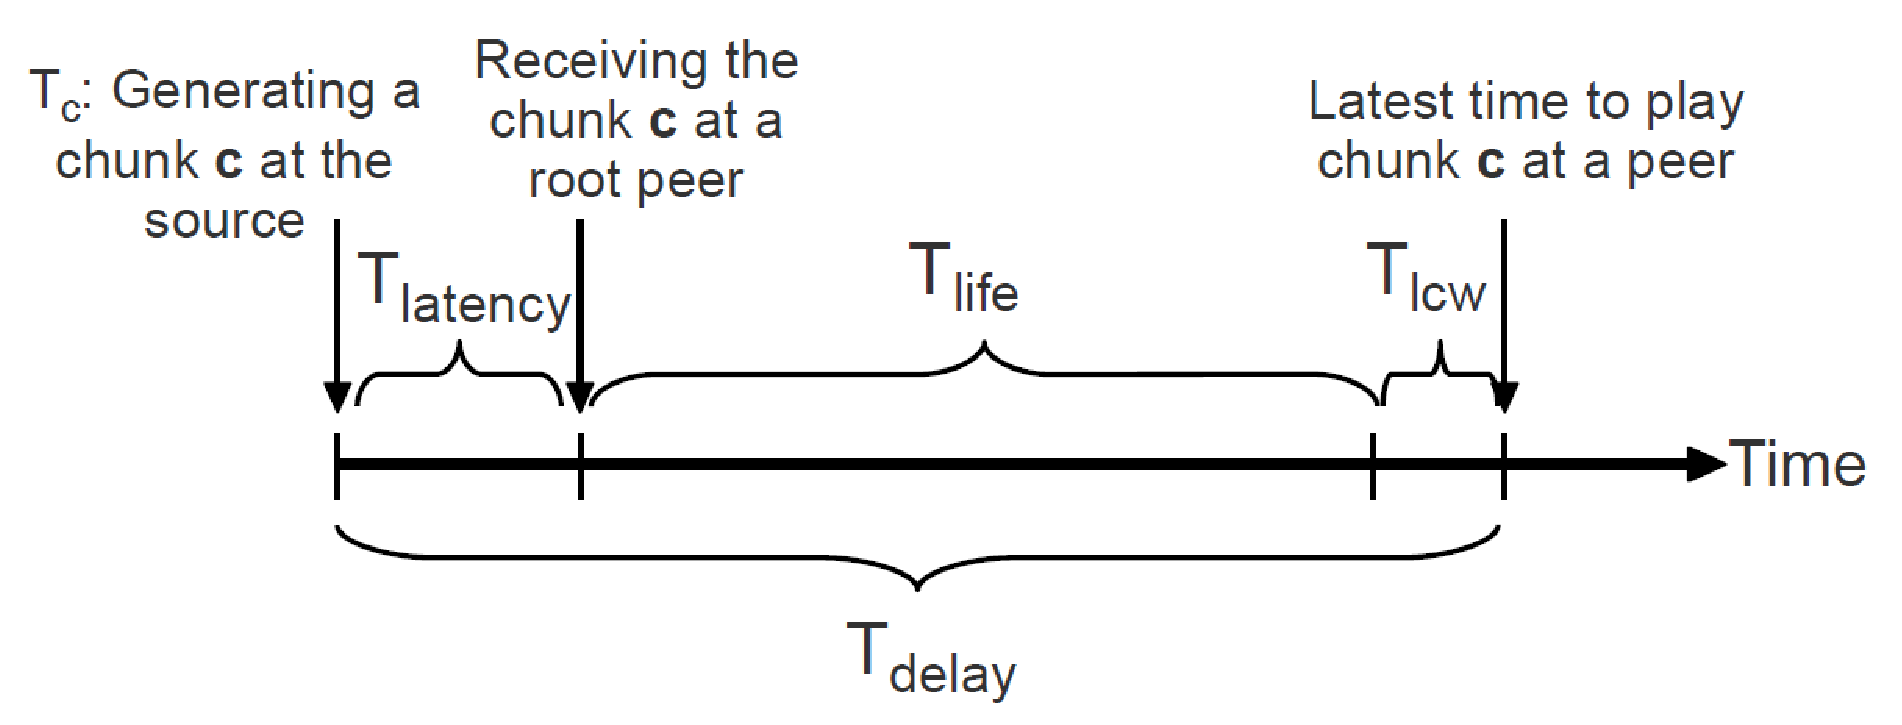
\includegraphics[width=1.0\columnwidth, trim=0 70 0 0]{tlife}
\vspace{3mm}
\caption{\small Live streaming time model.}
\label{fig:tlife}
\end{figure}

Therefore, a chunk $c$ generated at time $t(c)$ at the source must be played
at peers no later than $t(c) + \tdelay$, otherwise the QoS contract will be
violated. Moreover, the chunk $c$ becomes available at root peers by time
$t(c) + \tlatency$, and it should be available in the local buffer of any peer
in the swarm by time $t(c) + \tdelay - \tlcw$, otherwise the chunk will be
downloaded from the PH (Figure~\ref{fig:tlife}). This means that the lifetime
$\tlife$ of a chunk at root peers is equal to:
\begin{equation}
\tlife = (\tdelay - \tlatency) - \tlcw \label{tlife}
\end{equation}

Whenever a root peer $r$ receives a chunk $c$ for the first time, it starts
disseminating it in the swarm. Biskupski et al. in \cite{treebasedmesh} show
that a chunk disseminated by a pull mechanism through a mesh overlay follows a
tree-based diffusion pattern. We recursively define the {\em diffusion tree} $DT(r, c)$
rooted at a root peer $r$ of a chunk $c$ as the set of peers, such that a peer
$q$ belongs to $DT(r, c)$, if it has received $c$ from a peer $p \in DT(r, c)$.

Learning the exact diffusion tree for all chunks is difficult, because this
would imply a global knowledge of the overlay network and its dynamics, and
each chunk may follow a different tree. Fortunately, such precise knowledge is
not needed. What we would like to know is an estimate of the number of peers
that can be theoretically reached through the source or the current population
of AHs.

The chunk generation execution is divided into rounds of length $\tround$.
Chunk uploaded at round $i$ becomes available for upload to other peers at
round $i+1$. The maximum depth, $\Depth$, of any diffusion tree of a chunk
over its $\tlife$ is computed as: $\Depth = \lfloor \tlife / \tround \rfloor$.
We assume that $\tround$ is bigger than the average latency among the peers in
the swarm. Given $\Depth$ and the probability density function $P_{\omega}$,
we define the procedure $\treesize(P_{\omega}, \Depth)$ that executes locally
at the CM and provides an estimate of the number of peers of a single diffusion
tree (Algorithm~\ref{src:infected}). This algorithm emulates a large number of
diffusion trees, based on the probability density function $P_{\omega}$, and
returns the smallest value obtained in this way.

Emulation of a diffusion tree is obtained by the recursive procedure
$\treesizerec(P_{\omega}, \Depth)$. In this procedure, variable $n$ is
initialized to $1$, meaning that this peer belongs to the tree. If the depth
of the tree is larger than $0$, another round of dissemination can be
completed. The number of upload slots is drawn randomly by function
$\Random()$ from the probability density function $P_{\omega}$. Variable $n$
is then increased by adding the number of peers that can be reached by
recursive call to $\treesizerec()$, where the depth is decremented by $1$ at
each step before the next recursion.
\begin{algorithm}[!ht]
\caption{Lower bound for the diffusion tree size.}
\label{src:infected}
\begin{scriptsize}
\PROCEDURE{size$(\Density\ P_{\omega}, \INTEGER\ \Depth)$}{
  \INTEGER\ $\Min \gets +\infty$\;
  \REPEAT{$k$}{
    $\Min \gets \MIN(\Min,$ recSize$(P_{\omega}, \Depth))$\;
  }
  \Return $\Min$;
}
\BlankLine
\PROCEDURE{recSize$(\Density\ P_{\omega}, \INTEGER\ \Depth)$}{
  \INTEGER $n \gets 1$\;
  \If{$\Depth > 0$}{
    \INTEGER $\Slots \gets \Random(P_{\omega})$\;
    \For{$i \gets 1$ \TO\ $\Slots$}{
      $n \gets n +$ recSize$(P_{\omega}, \Depth-1)$\;
    }
  }
  \Return $n$\;
}
\end{scriptsize}
\end{algorithm}

At this point, the expected number of infected peers, i.e., the total peers
that can receive a chunk directly or indirectly from AHs and the source, but
not from the PH, $\Nexp$, is given by the total number of root peers times the
estimated diffusion tree size, $\Ntree = \treesize(P_{\omega}, depth)$. The
number of root peers is computed as the sum of the upload slots at the
source, $\UpSlots{s}$, and AHs, $\UpSlots{h}$, minus the number of slots used to
push chunks to the AHs themselves, as well as to the PH, which is equal to the
number of AHs plus one. Considering $\AH$ as the set of all AHs, we have:
\begin{equation}\label{eq:n}
  \Nexp = \left(\UpSlots{s} + \sum_{h \in \mathit{\AH} } \UpSlots{h} - \left( |\AH| + 1 \right) \right) \cdot \Ntree 
\end{equation}

\subsection{The management model} \label{ahmgt}
We define the cost $\Cah$ of an AH in one round ($\tround$) as the following:
\begin{equation}\label{eq:ahcost}
\Cah = \Cvm + m \cdot \Ctransfer
\end{equation}
where $\Cvm$ is the cost of running one AH (virtual machine) in a round,
$\Ctransfer$ is the cost of transferring one chunk from an AH to a peer, and
$m$ in the number of chunks that one AH uploads per round. Since we utilize
all the available upload slots of an AH, we can assume that $m = \UpSlots{h}$.
Similarly, the cost $\Cph$ of pulling chunks from PH per round is:
\begin{equation}\label{eq:phcost}
\Cph = \Cstorage + r \cdot (\Ctransfer + \Creq) 
\end{equation}
where $\Cstorage$ is the storage cost, $\Creq$ is the cost of retrieving (GET)
one chunk from PH and $r$ is the number of chunks retrieved from PH per round.
$\Ctransfer$ of PH is the same as in AH. Moreover, since we store only a few
minutes of the live stream in the storage, $\Cstorage$ is negligible.
\begin{figure}[t]
\centering
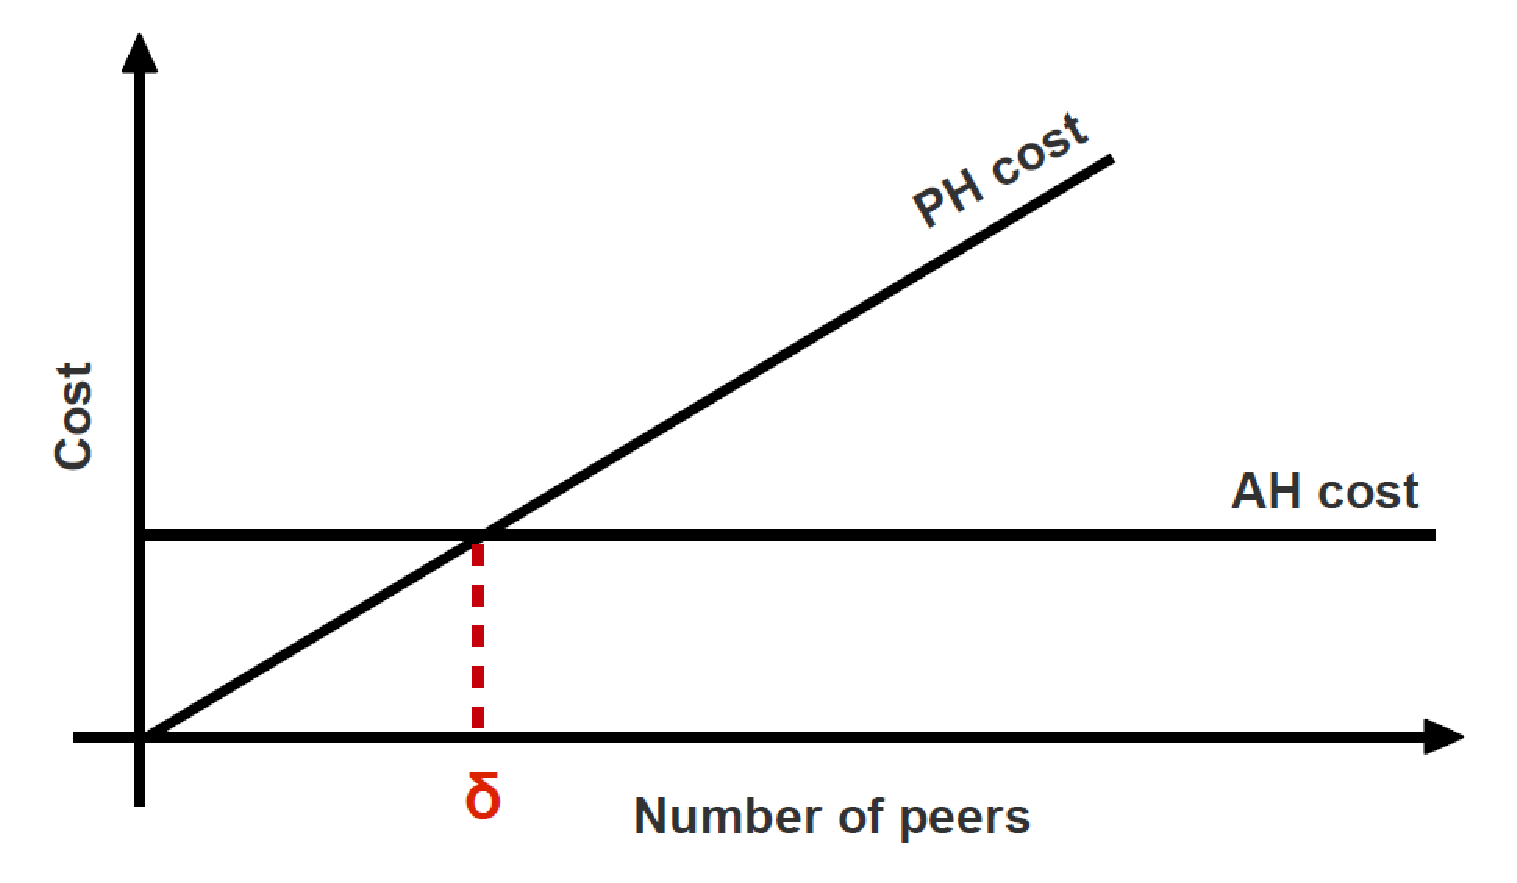
\includegraphics[width=0.7\columnwidth,]{delta}
\caption{\small Calculating the number of peers that is economically reasonable to serve with PH utilization instead of running an additional AH.}
\label{fig:delta}
\end{figure}

Figure~\ref{fig:delta} shows how $\Cah$ and $\Cph$ (depicted in
Formulas~\ref{eq:ahcost} and~\ref{eq:phcost}) changes in one round
($\tround$), when the number of peers increases. We observe that $\Cph$
increases linearly with the number of peers (number of requests), while $\Cah$
is constant and independent of the number of peers in the swarm. Therefore, if
we find the intersection of the cost functions, i.e., the point $\delta$ in
Figure~\ref{fig:delta}, we will know when is economically reasonable to add a
new AH, instead of putting more load on PH.
\begin{equation}\label{eq:delta}
\delta \approx \frac{\Cvm + m \cdot \Ctransfer}{\Ctransfer + \Creq}
\end{equation}

The CM considers the following thresholds and regulation behavior:
\begin{itemize}
\item $\Nswarm > \Nexp + \delta$: This means that the number of peers in the swarm is larger than the maximum size that can be served with a given configuration, thus, more AHs should be added to the system. 
\item $\Nswarm < \Nexp + \delta - \UpSlots{h} \cdot \Ntree$: Current configuration is able to serve more peers than the current network size, thus, extra AHs can be removed. $\UpSlots{h} \cdot \Ntree$ shows the number of peers served by one AH. 
\item $\Nexp + \delta - \UpSlots{h} \cdot \Ntree \leq \Nswarm \leq \Nexp + \delta$: In this interval the system has adequate resource and no change in the configuration is required.
\end{itemize}

The CM periodically checks the above conditions, and takes the necessary actions,
if any. In order to prevent temporary fluctuation, it adds/removes only single
AH in each step.

\subsection{Discussion} \label{lcw}

$\tlcw$ is a system parameter that has an important impact on the quality of
the received media at end users, as well as on the total cost. Finding an
appropriate value for $\tlcw$ is challenging. With $\tlcw$ a too small, peers
may fail to fetch chunks from PH in time for playback, while 
$\tlcw$ a too large increases the number of requests to PH, thus, increases the cost.
Therefore, the question is how to choose a value for $\tlcw$ to achieve (i)
the best QoS with a (ii) minimum cost.

\subsubsection{Impact of $\tlcw$ on the QoS} 

As we mentioned in Section~\ref{sec:system}, each peer buffers a number of
chunks ahead of its playback time, to guarantee a given level of QoS. The
number of buffered chunks corresponds to a time interval of length $\tlcw$.
The length of $\tlcw$ should be chosen big enough, such that if a chunk is not
received through other peers, there is enough time to send a request to PH and
retrieve the missing chunk from it in time for playback.

The required time for fetching a chunk from the PH depends on the round trip
time ($\rtt$) between the peer and the PH, and thus it is not the same for all the
peers. Therefore, each peer measures $\rtt$ locally, which consists of the
latency to send the request to the PH, plus the latency to receive the chunks at
the peer's buffer. A peer should send a request for a missing chunk to PH no
later than $\rtt$ time units before the playback time, otherwise, the retrieved chunk is
useless. Therefore, each peer sets the minimum value of $\tlcw$ to $\rtt$.

While $\tlcw$ is a local value at each peer, $\tlife$, which is used by the CM to
calculate the number of infected peers, depends on $\tlcw$
(Equation~\ref{tlife}). Therefore, the CM should be aware of the average $\tlcw$
among peers. To provide this information to the CM, all peers, including the CM,
participate in an aggregation protocol to get the average of $\tlcw$ among all
peers. Algorithm~\ref{src:shuffle_view} shows that in each shuffle, a peer
sends its local $\tlcw$ to other peers, and upon receiving a reply it updates
its $\tlcw$ to the average of its own $\tlcw$ and the received one.

\subsubsection{Impact of $\tlcw$ on the cost} 

Equation~\ref{eq:phcost} shows that the cost of PH increases linearly with
the  number of requests in each round. On the other hand, increasing
$\tlcw$ increases the PH cost in a round, as peers send more requests to PH.
To have a more precise definition of PH cost in Equation~\ref{eq:phcost}, we
replace $r$, which is the number of received requests at PH, with $\delta
\times l$, where $l$ is the normalized value of $\tlcw$ at the CM by the average
$\tlcw$ (achieved in the aggregation protocol), i.e., $l =
\frac{\tlcw}{\textrm{avg}\tlcw}$, and $\delta$ is the number of peers sending
requests to PH in a round. Therefore, Equation~\ref{eq:delta} can be rewritten
as follows:
\begin{equation}\label{eq:newdelta}
\delta \approx \frac{\Cvm + m \cdot \Ctransfer}{l \times (\Ctransfer + \Creq)}
\end{equation}

The CM uses the average $\tlcw$ to tune $\tlcw$ of the system. If the CM finds out
that changing $\tlcw$ can decrease the cost, without violating the QoS, it
floods the new value of $\tlcw$ to the peers. To do that, it sends the new
$\tlcw$ to the directly connected peers, and each peer forwards it to all its
neighbors, expect the one that it receives the message from. In the flooding
path, the peers with smaller $\tlcw$ than the received one update their local
$\tlcw$. However, if $\tlcw$ at a peer is bigger than the received value, it
does not change it, as its current $\tlcw$ is the minimum required time to get
a chunk from PH. Note that in Equation~\ref{eq:delta}, we assumed the local CM
$\tlcw$ equals the aggregated average of $\tlcw$, thus, $l=1$.

Figure~\ref{fig:delta} shows the relation between $\tlcw$ and PH cost.
The higher $\tlcw$ is, the steeper the PH cost line is. This 
means that the cost of PH increases faster when 
$\tlcw$ is large, since PH receives more requests in a shorter time. Moreover,
smaller values for $\tlcw$ push the PH cost line toward the x-axis. For
example, if $\tlcw$ is zero, i.e., peers never use the PH, the associated  cost is zero and
the line overlaps the x-axis. However, we cannot set $\tlcw$ to zero, since we
use PH as a backup of the chunks to guarantee the promised QoS.

Increasing $\tlcw$ not only increases the PH cost, but also increases the
total system cost. We see in Section~\ref{ahmgt}, that the CM uses two parameters to
manage the AHs, (i) the value of $\delta$, and (ii) the number of infected
peers. As Equation~\ref{eq:newdelta} shows, the higher $\tlcw$ is, the smaller
$\delta$ is. On the other hand, according to Equation~\ref{tlife}, increasing
$\tlcw$ decreases $\tlife$, and consequently, decreases the number of infected
peers. Hence, increasing $\tlcw$, decreases both $\delta$, and number of
infected peers, and as a result the CM adds more AHs to the system, according to
the management model in Section~\ref{ahmgt}, which increases the total cost.

To summarize, we can say that the best value for $\tlcw$ is the aggregated
average $\tlcw$, where $l = 1$. Decreasing $\tlcw$ below the average $\tlcw$,
i.e., $l < 1$, decreases the QoS at peers, as they may fail to fetch chunks
from PH before their playback time. On the other hand, although increasing
$\tlcw$ may increase QoS, it also increases the cost ($l > 1)$. Hence, the CM
never broadcasts new value of $\tlcw$ to the system.

\section{Experiments} \label{sec:evaluation}

In this section, we evaluate the performance of \clive using
\kompics~\cite{kompics}, a framework for building P2P protocols that provides
a discrete event simulator for testing the protocols using different
bandwidth, latency and churn scenarios.

\begin{table}[!ht]
\caption{\small Slot distribution in freerider overlay.}
\begin{center}
\begin{tabular}{| c | c |}
 \hline
  Number of slots & Percentage of peers \\ \hline \hline
  0 & 49.3\% \\ \hline
  1 & 18.7\% \\ \hline
  2 & 8.4\% \\ \hline
  3-19 & 5.2\% \\ \hline
  20 & 6.8\% \\ \hline
  Unknown & 11.6\% \\ \hline
  \end{tabular}
\label{tb:slotdist}
\end{center}
\end{table}

\subsection{Experimental setting}

In our experimental setup, we set the streaming rate to $500$kbps, which is divided into chunks of $20$kb; each chunk, thus, corresponds to $0.04$s of video stream. We define the {\em slot} as the unit of transferring the chunks, and based on that we define the upload bandwidth and download bandwidth at peers. The upload bandwidth of a peer is measured as ${\tt (num\ of\ upload\ slots) \times (slot\ bandwidth)}$. Similarly, we can measure the download bandwidth. For example, if the slot bandwidth is $100$kbps, then, the upload bandwidth of a peer with 5 upload slots would be $500$kbs.

Without loss of generality, we assume all
peers have enough download bandwidth to receive the stream with the correct
rate. In these experiments, all peers have $8$ download slots, and we consider
three classes of upload slot distributions: (i) {\em homogeneous}, where all
peers have $8$ upload slots, (ii) {\em heterogeneous}, where the number of
upload slots in peers is picked uniformly at random from $4$ to $13$, and
(iii) {\em real trace} (Table~\ref{tb:slotdist}) based on a study of large
scale streaming systems~\cite{Sripanidkulchai}. As it is shown in
Table~\ref{tb:slotdist}, around $50$\% of the peers in this model do not
contribute to the data distribution. We set the slot bandwidth to $100$kbps in our experiments. The media source is a single node that
pushes chunks to $10$ other peers. We assume PH has infinite upload bandwidth,
and each AH can push chunks to $20$ other peers. 

There are a number of studies on the impact of chunk size on the playback continuity of peers that show that the smaller the chunk size is, the higher playback continuity peers have~\cite{sepidar,newcoolstreaming}. In our experiments, we use the chunk size similar to the chunk size used in real systems, like BitTorrent, which is $16$kb. However, since we assume that the slot bandwidth is $100$kbps in our experiments, we chose $20$kb instead of $16$kb just to get whole (round) numbers after the division. Peers start playing the media after buffering it for $15$ seconds, which is comparable to the buffering time in SopCast, the most widely deployed P2P live streaming system~\cite{sopcast,fallica2008quality}. $\tdelay$ also equals $25$ seconds. Latencies between peers are modeled using a latency map based on the King data-set~\cite{king}.

\begin{figure}[t]
\centering
\includegraphics[angle=270, width=0.47\columnwidth,]{fig-pc-join}\label{fig:pc-join}
\vspace{-2pt}
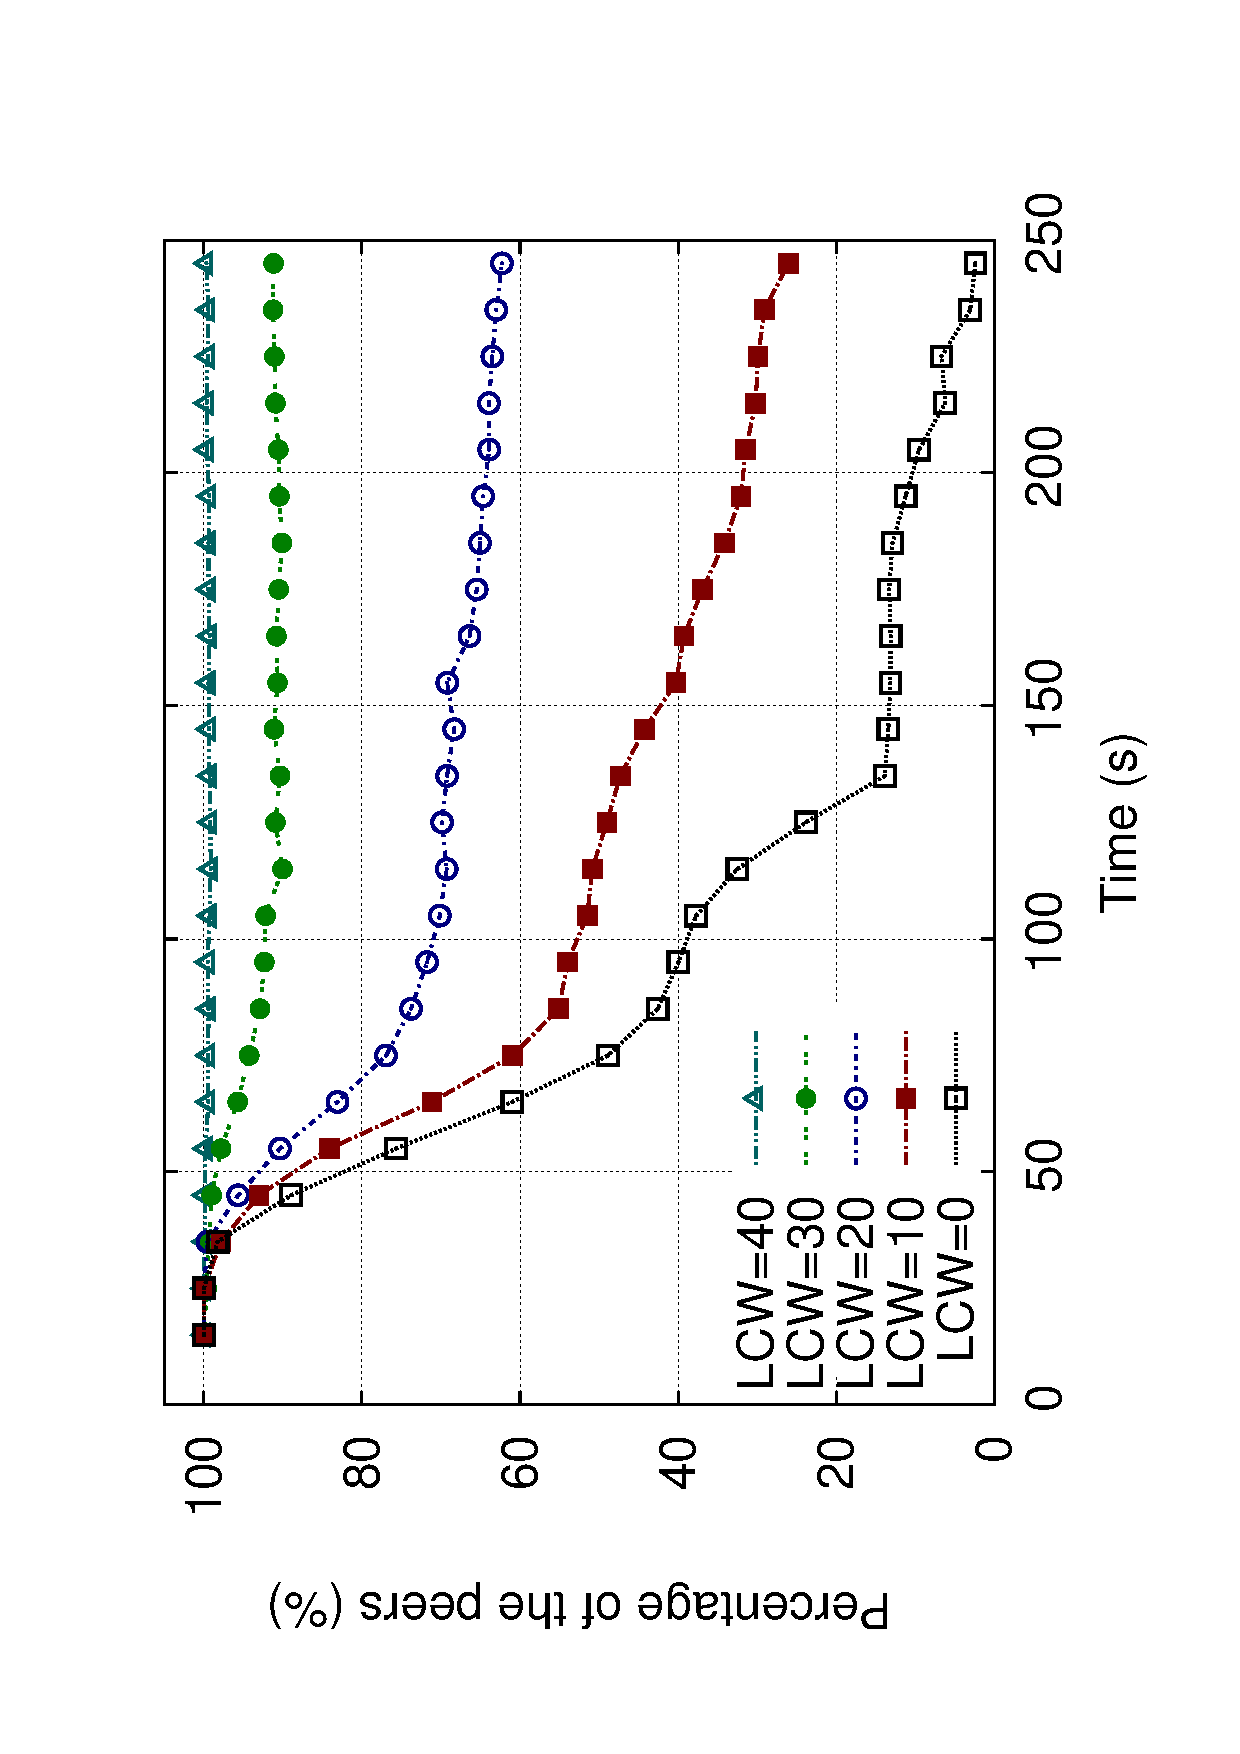
\includegraphics[angle=270, width=0.47\columnwidth]{fig-pc-churn}\label{fig:pc-churn}
\caption{\small The percentage of the peers receiving 99\% playback continuity with different values of $\tlcw$ (measured in number of chunks). Top: join scenario, bottom: churn scenario ($1\%$ churn rate).}
\label{fig:pc}
\end{figure}

In our experiments, we used two failure scenarios: {\em join-only} and {\em
churn}. In the join-only scenario, $1000$ peers join the system following a
Poisson distribution with an average inter-arrival time of $10$ milliseconds,
and after joining the system they will remain till the end of the simulation.
In the churn scenario, approximately $0.01$\%, $0.1$\% and $1$\% of the peers
leave the system per second and rejoin immediately as newly initialized
peers~\cite{churn}. However, unless stated otherwise, we did the experiments
with $1\%$ churn rate to show how the system performs in presence of high
dynamism. {A continuous churn of more than $1\%$ is simply unrealistic. Well, already $1\%$ is unrealistic: it means that the average life time of nodes is less than 2 minutes, which means continuous zapping. At that point, no P2P network could help with that.

To the best of our knowledge, \clive is the only system that uses both PH and AH from a cloud provider for live streaming and studies their impact on the cost and performance. The existing systems consider only PH, as in CloudCast~\cite{cloudcast} and CloudMedia~\cite{cloudmedia}, or only AHs, as in AngelCast/CloudAngel~\cite{angelcast}, and they are designed for content distribution or video on demand. However, \clive is a live streaming system with real-time constraints on data delivery, which is not considered in the previous systems. Therefore, in this section we compare \clive with the baseline model, which is similar to the systems that use only PH.

\subsection{The effect of $\tlcw$ on system performance}

In the first experiment, we evaluate the system behavior with different values
for $\tlcw$, measured in number of chunks. In this experiment, we measure {\em
playback continuity} and {\em playback delay}, which combined together reflect
the QoS experienced by the overlay peers. Playback continuity shows the
percentage of chunks received on time by peers, and playback delay represents
the difference, in seconds, between the playback point of a peer and the
source.
\begin{figure}[t]
\centering
\includegraphics[angle=270, width=0.47\columnwidth,]{fig-pl-join}\label{fig:pl-join} 
\includegraphics[angle=270, width=0.47\columnwidth,]{fig-pl-churn}\label{fig:pl-churn}
\caption{\small Average playback delay across peers with different values of $\tlcw$ (measured in number of chunks). Top: join scenario, bottom: churn scenario ($1\%$ churn rate).}
\label{fig:pl}
\end{figure}

\begin{figure*}[t]
\centering
\subfigure[\scriptsize Join-only.]{\includegraphics[angle=270, width=0.47\columnwidth,]{fig-ph-load-join}\label{fig:ph-load-join}}
\subfigure[\scriptsize Churn ($1\%$ churn rate).]{\includegraphics[angle=270, width=0.47\columnwidth,]{fig-ph-load-churn}\label{fig:ph-load-churn}}\\
\subfigure[\scriptsize Different churn rates ($LCW=40$ chunks).]{\includegraphics[angle=270, width=0.47\columnwidth,]{fig-ph-load-churn-rate}\label{fig:ph-load-churn-rate}}
\subfigure[\scriptsize Different churn rates at root peers ($LCW=40$ chunks).]{\includegraphics[angle=270, width=0.47\columnwidth,]{fig-ph-load-rootpeer}\label{fig:ph-load-rootpeer}}
\caption{\small The cumulative PH load with different values of $\tlcw$ and churn rates.}
\label{fig:ph-load}
\end{figure*}

For a cleaner observation of the effect of $\tlcw$, we use the homogeneous
slot distribution in this experiment. Figure~\ref{fig:pc} shows the fraction
of peers that received at least $99\%$ of the chunks before their timeout with
different $\tlcw$ in the join-only and churn scenarios ($1\%$ churn rate). We
changed $LCW$ between $0$ to $40$ chunks, where zero means peers never use PH,
and $40$ means that a peer retrieves up to chunk $c+40$ from PH, if the peer
is currently playing chunk $c$. As we see, the bigger $\tlcw$ is, the more
peers receive chunks in time. Although for any value of $\tlcw>0$ peers try to
retrieve the missing chunks from PH, the network latency may not allow to
obtain the missing chunk in time. As Figure~\ref{fig:pc} shows, all the peers
retrieve 99\% of the chunks on time when $LCW=40$. Given that each chunk
corresponds to $0.04$ seconds, $\tlcw=40$ implies $1.6$ seconds.

The average playback delay of peers is shown in Figure~\ref{fig:pl}. In the
join-only scenario, playback delay does not depend on $\tlcw$, while in the
churn scenario we can see a sharp increase when $\tlcw$ is small.

\subsection{PH load in different settings}
We then measured the PH load or the amount of fetched chunks from PH with
different $\tlcw$ values and churn rates. Figures~\ref{fig:ph-load-join}
and~\ref{fig:ph-load-churn} show the cumulative load of PH in the join-only
and churn scenarios ($1\%$ churn rate), respectively. As we see in these
figures, by increasing $\tlcw$, more requests are sent to PH, thus, increasing
its load. Figure~\ref{fig:ph-load-churn-rate} depicts the cumulative PH load
over time for four different churn rates and $LCW$ equals 40 chunks. As the
figure shows, there is no big change in PH load under low churn scenarios
($0.01\%$ and $0.1\%$), which are deemed realistic in deployed P2P
systems~\cite{churn}. However, it sharply increases in the presence of higher
churn rates ($1\%$), because peers lose their neighbors more often, thus, they
cannot pull chunks from the swarm in time, and consequently they have to fetch
them from PH.

Moreover, we conducted an experiment to show the effect of failure of root peers (Figure~\ref{fig:ph-load-rootpeer}). We consider three scenarios, where $10\%$, $50\%$ and $100\%$ of root peers fail. We observed that in these failures, all the peers in the swarm receive chunks without any interruption, because in the worst case, when they lose all their partners, they pull the chunks from the PH. Figure~\ref{fig:ph-load-rootpeer} shows the PH load in these scenarios. As we see, when $10\%$ and $50\%$ of root peers fail, the PH load increases for a short time, but it goes back quickly to the situation before the failure. However, when all root peers fail, the PH load remains a bit more than the situation before the failure. In this scenario, many peers cannot receive chunks from the swarm at the right speed, thus, the number of buffered chunks at those peers decreases. These peers have shorter time to fetch chunks from other peers afterwards, therefore, they refer to the PH more 
often, even after resolving the failure.

\subsection{Economic cost}
In this experiment, we measure the effect of adding and removing AHs on the
total cost. Note, in these experiments we set $LCW$ to $40$ chunks, therefore,
regardless of the number of AHs, all the peers receive $99$\% of the chunks
before their playback time. In fact, AHs only affect the total cost of the
service. In Section~\ref{sec:cmmanager}, we showed how CM estimates the
required number of AHs. Figure~\ref{fig:ah} depicts how the number of AHs
changes over time. In the join-only scenario and the homogeneous slot
distribution (Figure~\ref{fig:ah-homo}), the CM estimates the exact value of
the peers that receive the chunks on time using the existing resources in the
system, and consequently the exact number of required AHs. Hence, as it is
shown, the number of AHs will be fixed during the simulation time. However, in
the heterogeneous and real trace slot distributions (Figures~\ref{fig:ah-hete}
and \ref{fig:ah-real}), CM estimation changes over time, and based on this, it
adds and removes AHs. In the churn scenario ($1\%$ churn rate), CM estimation
also changes over the time, thus, the number of AHs fluctuates.

\begin{figure*}[t]
\centering
\subfigure[\scriptsize Homogeneous.]{\includegraphics[angle=270, width=0.47\columnwidth,]{fig-ah-homo}\label{fig:ah-homo}}\\
\subfigure[\scriptsize Heterogeneous.]{\includegraphics[angle=270, width=0.47\columnwidth,]{fig-ah-hete}\label{fig:ah-hete}}
\subfigure[\scriptsize Real trace.]{\includegraphics[angle=270, width=0.47\columnwidth,]{fig-ah-real}\label{fig:ah-real}}
\caption{\small Number of AHs in different settings and scenarios.}\label{fig:ah}
\end{figure*}

\begin{figure*}[t]
\centering
\subfigure[\scriptsize Homogeneous.]{\includegraphics[angle=270, width=0.47\columnwidth,]{fig-ph-load-ah-homo}\label{fig:ph-load-homo}}\\
\subfigure[\scriptsize Heterogeneous.]{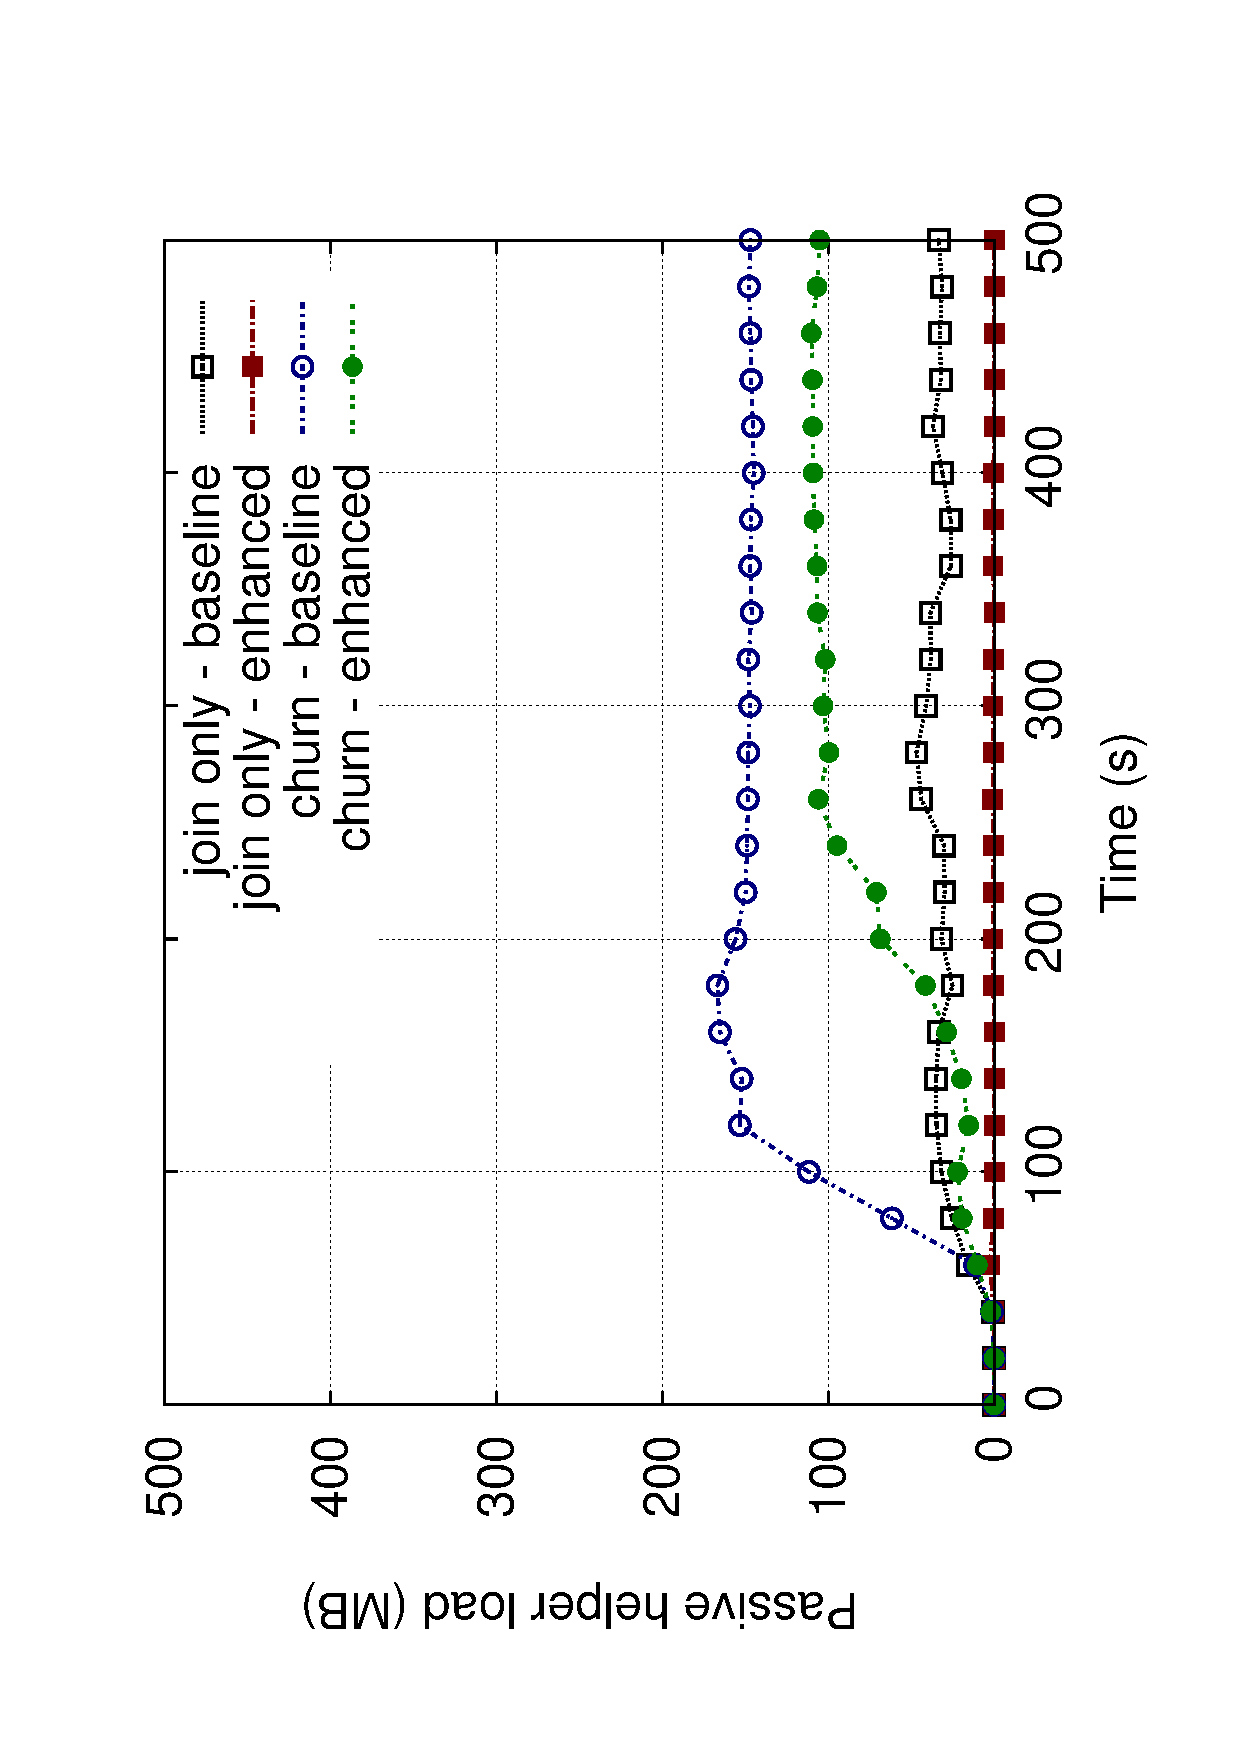
\includegraphics[angle=270, width=0.47\columnwidth,]{fig-ph-load-ah-hete}\label{fig:ph-load-hete}}
\subfigure[\scriptsize Real trace.]{\includegraphics[angle=270, width=0.47\columnwidth,]{fig-ph-load-ah-real}\label{fig:ph-load-real}}
\caption{\small PH load in different scenarios with dynamic changes of the number of AHs.}
\label{fig:ph-load-cost}
\end{figure*}

\begin{figure*}[t]
\centering
\subfigure[\scriptsize Homogeneous.]{\includegraphics[angle=270, width=0.47\columnwidth,]{fig-cost-homo}\label{fig:cost-homo}}\\
\subfigure[\scriptsize Heterogeneous.]{\includegraphics[angle=270, width=0.47\columnwidth,]{fig-cost-hete}\label{fig:cost-hete}}
\subfigure[\scriptsize Real trace.]{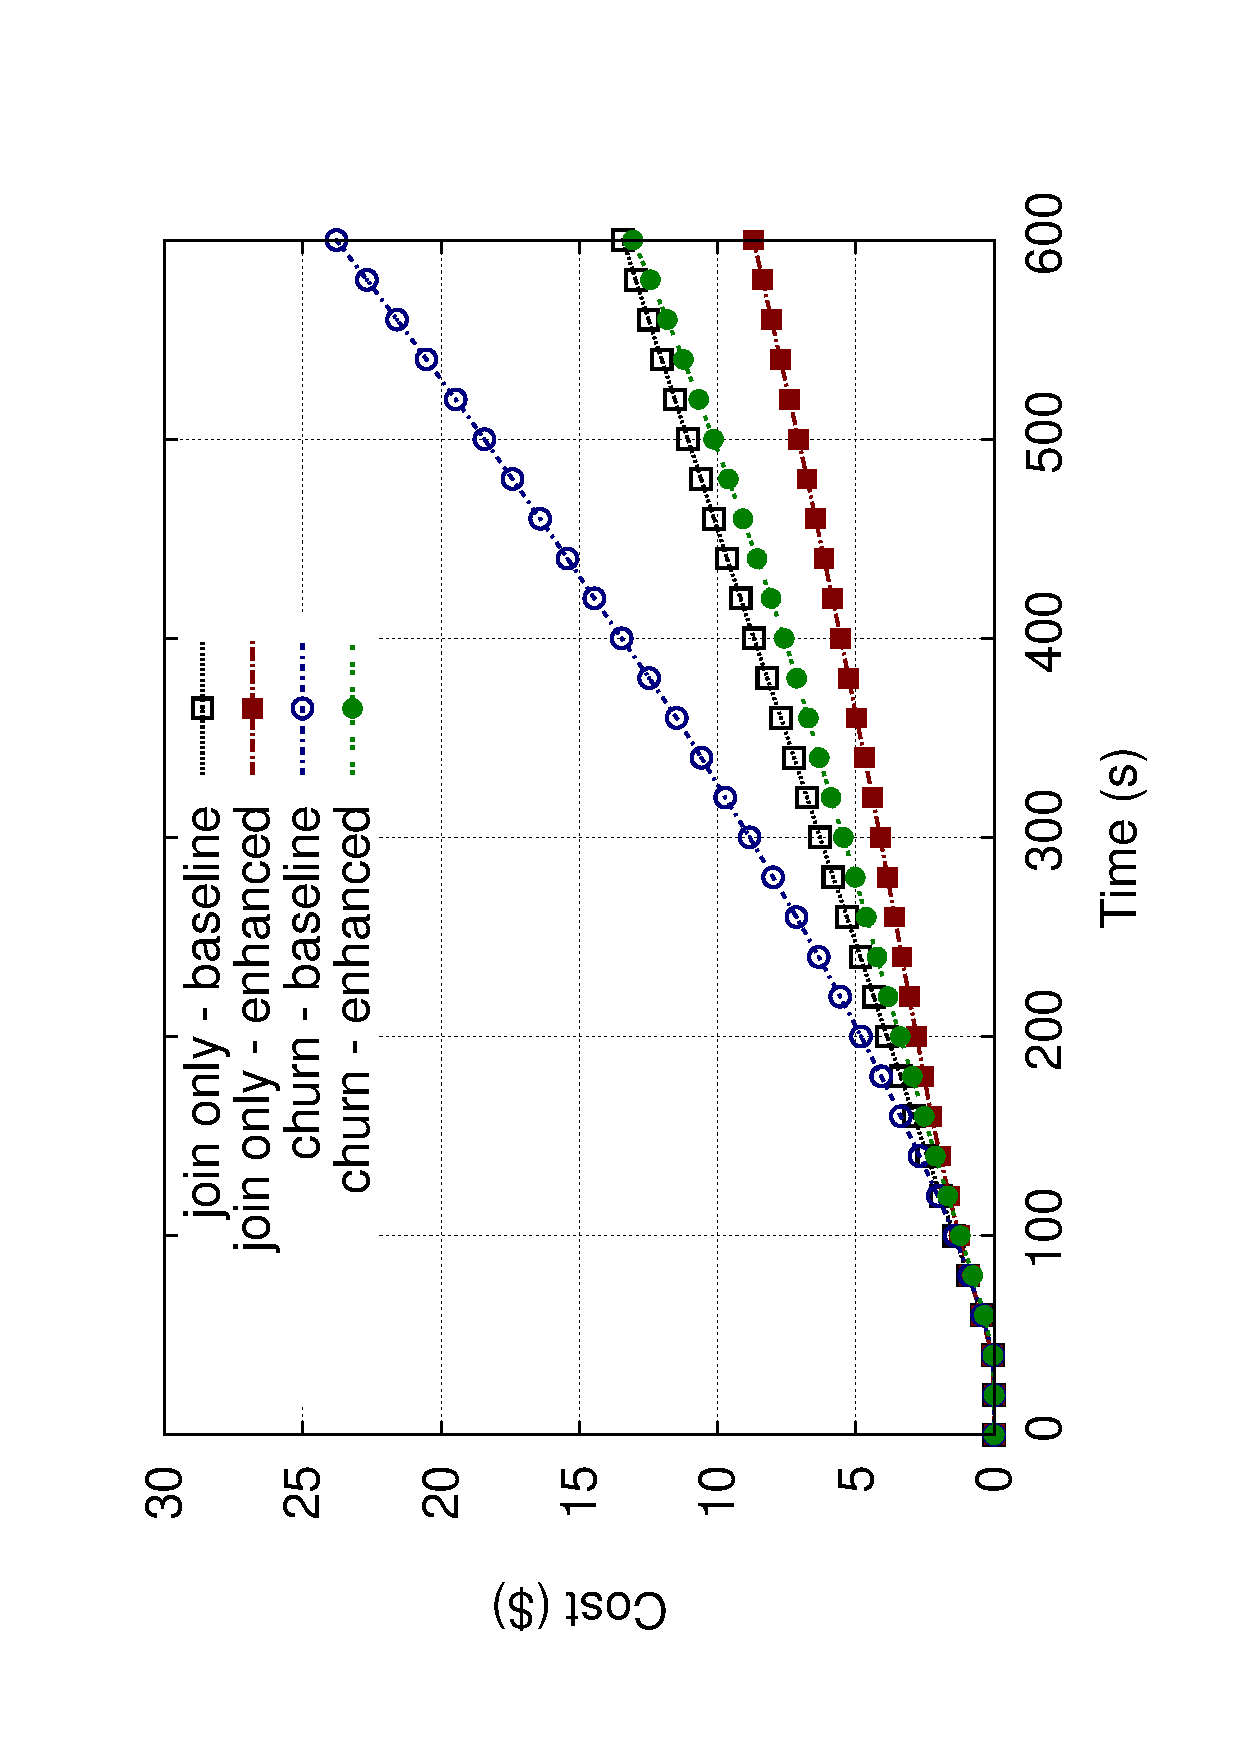
\includegraphics[angle=270, width=0.47\columnwidth,]{fig-cost-real}\label{fig:cost-real}}
\caption{\small The cumulative total cost for different setting and scenarios.}
\label{fig:cost}
\end{figure*}

Relatively, we see how PH load changes in different scenarios in the baseline
and enhanced models (Figure~\ref{fig:ph-load-cost}). Figure~\ref{fig:ah-homo}
shows that three AHs are added to the system in the join-only scenario and the
homogeneous slot distribution. On the other hand, we see in
Figure~\ref{fig:ph-load-homo}, in the join-only scenario, with the help of
these three AHs (enhanced model), the load of PH goes down nearly to zero. It
implies that three AHs in the system are enough to minimize PH load, while
preserving the promised level of QoS. Hence, adding more than three AHs in
this setting does not have any benefit and only increases the total cost.
Moreover, we can see in the join-only scenario, if there is no AH in the
system (baseline model), PH load is much higher than the enhanced model, e.g.,
around $90mb$, $40mb$, and $130mb$ per second in the homogeneous,
heterogeneous, and real trace, respectively. The same difference appears in
the churn scenario.

Figure~\ref{fig:cost} shows the cumulative total cost over the time in
different scenarios and slot distributions. In this measurement, we use Amazon
S3 as PH and Amazon EC2 as AHs. According to the price list of
Amazon~\cite{amazonec2,amazons3}, the data transfer price of S3 is 0.12\$ per
GB, for up to 10 TB in a month. The cost of GET requests are 0.01\$ per 10000
requests. Similarly, the cost of data transfer in EC2 is 0.12\$ per GB, for up
to 10 TB in a month, but since the AHs actively push chunks, there is no GET
requests cost. The cost of a large instance of EC2 is 0.34\$ per hour.

Considering the chunk size of $20kb$ ($0.02mb$) in our settings, we can
measure the cost of PH in Amazon S3 per round (second) according to the
Formula~\ref{eq:phcost}:
\begin{eqnarray}
\Cph &\approx& r \cdot (\Ctransfer + \Creq) \nonumber \\
&\approx& \frac{r \times 0.02 \times 0.12}{1000} + \frac{r \times 0.01}{10000}
\end{eqnarray}

where $r$ is the the number of received requests by PH in one round (second).
The cost of storage is negligible. Given that each AH pushes chunks to 20
peers with the rate of $500kbps$ ($0.5mbps$), then the cost of running one AHs
in Amazon EC2 per second according to Formula~\ref{eq:ahcost} is:
\begin{eqnarray}
\Cah &=& \Cvm + m \cdot \Ctransfer \nonumber \\
&=& \frac{0.34}{3600} + \frac{20 \times 0.5 \times 0.12}{1000}
\end{eqnarray}

Figure~\ref{fig:cost} shows the cumulative total cost for different slot
distribution settings. It is clear from these figures that adding AHs to the
system reduces the total cost, while keeping the QoS as promised. For example,
in the high churn scenario ($1\%$ churn rate) and the real trace slot
distribution the total cost of system after $600$ seconds is $24$\$ in the
absence of AHs (baseline model), while it is close to $13$\$ if AHs are added
(enhanced model), which saves around $45\%$ of the cost.

\subsection{Accuracy evaluation}

In this section we evaluate the accuracy of our estimations in form of
evaluating the accuracy of upload slot distribution, and the accuracy of
estimating the number of infected peers.

\subsubsection{Upload slot distribution estimation}

Here, we evaluate the estimation of upload slots distribution in the system.
We adopt the Kolmogorov-Smirnov (KS) distance~\cite{schay2007introduction}, to
define the upper bound on the approximation error of any peer in the system.
The KS distance is given by the maximum difference between the actual slot
distribution, $\omega$, and the estimated slot distribution, $E(\omega)$. We
compute $E(\omega)$ based on $P_{\omega}$ for different number of slots. Since
the maximum error is determined by a single point (slot) difference between
$\omega$ and $E(\omega)$, it is sensitive to noise. Hence, we measure the
average error at each peer as the average error contributed by all points
(slots) in $\omega$ and $E(\omega)$. The total average error is then computed
as the average of these local average errors.

We consider three slot distributions in this experiment: (i) the uniform
distribution, (ii) the exponential distribution ($\lambda = 1.5$), and (iii)
the Pareto distribution ($k = 5, x_m = 1$). Figure~\ref{fig:slot-distro} shows
the average error in three slot distributions, and Figure~\ref{fig:slot-churn}
shows how the accuracy of the estimation changes in different churn rates.

\begin{figure}[h]
\centering
\subfigure[\scriptsize Avg. error in different slot distributions.]{\includegraphics[angle=270, width=0.47\columnwidth,]{fig-slot-distro}\label{fig:slot-distro}}
\subfigure[\scriptsize Avg. error in different churn rates.]{\includegraphics[angle=270, width=0.47\columnwidth,]{fig-slot-churn}\label{fig:slot-churn}}
\caption{\small Avg. estimation error.}
\label{fig:distro}
\end{figure}

\subsubsection{Number of infected peers estimation}
Finally, we evaluate the estimation accuracy of the number of infected peers.
Figure~\ref{fig:acc} shows the real number of infected peers and estimated
ones in three upload slot distributions and in join and churn scenarios. As
shown in the homogeneous and heterogeneous slot distributions, our estimation
of the number of infected peers closely fits the real number of such peer.
However, in the real trace slot distribution, it may happen that a peer
without upload slot connects directly to the source and prevents other peers
to join the system, or on the other hand, a very high upload bandwidth peer
joins close to the source and serves many other peers. That is why we see more
difference between the real and estimated number of infected peers in the real
trace slot distribution.

\begin{figure*}[t]
\centering
\subfigure[\scriptsize Homogeneous (join).]{\includegraphics[angle=270, width=0.47\columnwidth,]{fig-join-homo}\label{fig:acc-join-homo}}
\subfigure[\scriptsize Heterogeneous (join).]{\includegraphics[angle=270, width=0.47\columnwidth,]{fig-join-hete}\label{fig:acc-join-hete}}\\
\subfigure[\scriptsize Real trace (join).]{\includegraphics[angle=270, width=0.47\columnwidth,]{fig-join-real}\label{fig:acc-join-real}}
\subfigure[\scriptsize Homogeneous (churn).]{\includegraphics[angle=270, width=0.47\columnwidth,]{fig-churn-homo}\label{fig:acc-churn-homo}}\\
\subfigure[\scriptsize Heterogeneous (churn).]{\includegraphics[angle=270, width=0.47\columnwidth,]{fig-churn-hete}\label{fig:acc-churn-hete}}
\subfigure[\scriptsize Real trace (churn).]{\includegraphics[angle=270, width=0.47\columnwidth,]{fig-churn-real}\label{fig:acc-churn-real}}
\caption{\small The comparison between the real number of infected nodes and the estimated ones.}
\label{fig:acc}
\end{figure*}

\section{Related work} \label{sec:relatedwork}

\subsection{Hybrid approaches for content distribution}
Although P2P algorithms are emerging as promising solutions for large scale
content distribution, they are still subject to a number of
challenges~\cite{challenge}. A typical problem is the bottleneck in the
aggregated upload bandwidth in the overlay~\cite{Kumar:MDT} that can lead to a
low stream quality with disruptions. The bottleneck is caused by asymmetric
bandwidth of the clients: the download bandwidth is usually much higher than
upload.

In order to address these issues some recent research works propose to use an
hybrid architecture combining Content Delivery Networks (CDN) and
P2P overlays~\cite{ZhiHui_Lu,eue,Roverso_smoothcache}. Most of these works are focused on
reducing the use of CDN servers via utilization of P2P available resources
whenever it is possible. This kind of infrastructures is similar with the baseline
model considered in this paper. Instead we propose an enhanced
architecture that allows to regulate the amount of upload bandwidth in the
swarm via the utilization of additional cloud resources.

One of the most relevant works with respect to ours is LiveSky, developed by Yin et
al.~\cite{liveSky}. The authors proposed a commercial deployment of the hybrid
architecture, addressing several key challenges,
including dynamic resource scaling while guaranteeing stream quality. However,
while the authors consider redirection of the users according to available
upload resources, we propose an approach for managing the amount of available
upload bandwidth via swarm feedback processing.

%One more possible approach to increase the upload capacity is to use
%helpers~\cite{Wang:enchancing,Zhang:scaling}. The helper role can be played by
%{\em idle}~\cite{Wang:role} or {\em restricted}~\cite{Kumar2006} users. Idle
%users are peers with spare upload capacity that are not interested in any
%particular data, while restricted users are users with limited rights to use
%the network service. 

Nowadays, exploiting dedicated cloud servers to accelerate content distribution has become a very popular solution~\cite{CloudAngel,angelcast,budget}. 
In these systems, the role of the cloud servers is to cache and forward content to other peers. 
\angelcast~\cite{CloudAngel,angelcast} is a cloud-based live streaming acceleration service that combines P2P and cloud technologies, where the cloud entities play the role of helpers to build a multi-tree overlay for content distribution. Montresor and Abeni~\cite{cloudcast} introduced \cloudcast as a combination of P2P entities and passive cloud storage to support information diffusion in large scale P2P networks. They used Amazon S3 as dedicated server.

In addition to these solutions, Wu et al. proposed \cloudmedia~\cite{cloudmedia} for video on demand (VoD) systems. The authors describe a queuing model to predict the dynamic demands of the users of a P2P
VoD system providing elastic amounts of computing and bandwidth resources on the fly while minimizing the cost. Differently from \clive, the \cloudmedia relies on a tracker server that maintains the list of peers with buffered data chunks.

Similarly, Jin et al. presented a cloud-assisted system for P2P media streaming for
mobile peers~\cite{mobilecloud}. In this system, mobile users located in the same area share bandwidth resources among each other, while the cloud is responsible for storage and computing demanding tasks.


Unlike all the described solutions, our work exploits cloud computing and storage resources
as a collection of active and passive helpers. The combination of both types
of helpers together with an effective resource management, distinguishes our
approach from previous work.

\subsection{Self-monitoring and self-configuration systems}

\emph{Self-monitoring} and \emph{self-configuration} mechanisms are essential
to manage large, complex and dynamic systems in an effective way.
Self-monitoring detects the current states of system components, while
self-configuration is aimed to adapt system configuration according to the
received information.

Self-monitoring allows the system to have a view on its current utilization
and state. One of the popular approaches for monitoring P2P overlays is
decentralized aggregation~\cite{aggregation}. For example, \adam~\cite{adam2}
presents a gossip-based aggregation protocol to estimate the distribution of
attributes across peers. Similarly, Van Renesse and
Haridasan~\cite{gossipestimation} propose a distribution estimation mechanism,
which can be used to aggregate not only the values of different peers but also
how the values are ranked in relation with each others. Another system that
uses aggregation is \croupier~\cite{croupier}, which is a NAT-aware peer
sampling service and use aggregation protocol to estimate the ratio of open
peers in the network.

Self-configuration is the process of configuring components and
protocols autonomously according to specified goals, e.g., reliability and
availability~\cite{amoretti_autonomous,self,tman,kavalionak:iwsos12}. A relevant example of a
self-configuration mechanism is proposed by Kavalionak and
Montresor~\cite{kavalionak:iwsos12} that considers a replicated service on top of
a mixed P2P and cloud system. This protocol is able to self-regulate the
amount of cloud storage resources utilization according to available P2P
resources. However, the main goal of the proposed approach is to support a
given level of reliability, whereas in our work we are interested in an
effective data dissemination that allows to self-configure the amount of
active and passive cloud resources utilization.

\section{Conclusions} \label{sec:conclusion}

The main contribution of this paper is \clive, a P2P live streaming system
that integrates cloud resources (helpers), whenever the peer resources are not
enough to guarantee a predefined QoS with a low cost. Two types of helpers are
used in \clive, active helpers (virtual machines participating in the streaming
protocol) and passive helpers (represented by a storage service that
provides content on demand). \clive estimates the available capacity in the
system through a gossip-based aggregation protocol and provisions the required
resources (AHs/PHs) from the cloud provider w.r.t the dynamic behavior of the
users.
%
Moreover, despite of our previous \clive work, here we provide more deep analysis
and evaluation of the system parameters.

One of the promising directions to extend the current work is to apply 
additional cloud computing services into the system architecture.

In particular, Amazon's Cloudfront extends S3 by
replicating read-only content to a number of edge locations, in order
to put clients closer to the data and reduce the communication latency.
Altogether, these edge locations (currently there are $34$ of them around the
world) can be seen as a unique PH, from where chunks can be pulled. From the
point of view of the source, the interface remain the same: content is
originally pushed to S3 and from there is replicated across geographically
dispersed data centers.


%\bibliographystyle{plain}
\begin{thebibliography}{5}

\bibitem{amazonec2}
Amazon elastic compute cloud ({Amazon EC2}).
\newblock {http://aws.amazon.com/ec2/}, [Online; accessed 20-Nov-2012].

\bibitem{amazons3}
Amazon simple storage service ({Amazon S3}).
\newblock {http://aws.amazon.com/s3/}, [Online; accessed 20-Nov-2012].

\bibitem{amoretti_autonomous}
Michele Amoretti, Alessandro Grazioli, and Francesco Zanichelli.
\newblock An autonomic approach for p2p/cloud collaborative environments.
\newblock {\em Peer-to-Peer Networking and Applications}, pages 1--16, 2015.

\bibitem{kompics}
C.~Arad, J.~Dowling, and S.~Haridi.
\newblock Developing, simulating, and deploying peer-to-peer systems using the
  {Kompics} component model.
\newblock In {\em Proc. of ICST'09}, page~16. ACM, 2009.

\bibitem{armbrust2010view}
M.~Armbrust, A.~Fox, R.~Griffith, A.D. Joseph, R.~Katz, A.~Konwinski, G.~Lee,
  D.~Patterson, A.~Rabkin, I.~Stoica, et~al.
\newblock A view of cloud computing.
\newblock {\em Communications of the ACM}, 53(4):50--58, 2010.

\bibitem{self}
O.~Babaoglu and M.~Jelasity.
\newblock Self-* properties through gossiping.
\newblock {\em Philosophical Transactions of the Royal Society A: Mathematical,
  Physical and Engineering Sciences}, 366(1881):3747--3757, 2008.

\bibitem{treebasedmesh}
B.~Biskupski, M.~Schiely, P.~Felber, and R.~Meier.
\newblock Tree-based analysis of mesh overlays for peer-to-peer streaming.
\newblock In {\em Proc. of DAIS'08}, pages 126--139. Springer, 2008.

\bibitem{carlsson}
N.~Carlsson and D.~Eager.
\newblock Peer-assisted on-demand streaming of stored media using
  bittorrent-like protocols.
\newblock In {\em Proc. of NETWORKING'07}, pages 570--581. Springer, 2007.

\bibitem{croupier}
J.~Dowling and A.H. Payberah.
\newblock Shuffling with a {Croupier}: Nat-aware peer-sampling.
\newblock In {\em Proc. of ICDCS'12}, pages 102--111. IEEE, 2012.

\bibitem{fallica2008quality}
B.~Fallica, Y.~Lu, F.~Kuipers, R.~Kooij, and P.~Van~Mieghem.
\newblock On the quality of experience of sopcast.
\newblock In {\em Proc. of NGMAST'08}, pages 501--506. IEEE, 2008.

\bibitem{qoe}
R.~Fortuna, E.~Leonardi, M.~Mellia, M.~Meo, and S.~Traverso.
\newblock {QoE} in pull based {P2P-TV} systems: overlay topology design
  tradeoffs.
\newblock In {\em Proc. of P2P'10}, pages 1--10. IEEE, 2010.

\bibitem{gossip++}
D.~Frey, R.~Guerraoui, A.M. Kermarrec, and M.~Monod.
\newblock Boosting gossip for live streaming.
\newblock In {\em Proc. of P2P'10}, pages 1--10. IEEE, 2010.

\bibitem{goel2006data}
S.~Goel and R.~Buyya.
\newblock Data replication strategies in wide area distributed systems.
\newblock Technical report, Idea Group Inc., Hershey, PA, USA, 2006.

\bibitem{king}
K.P. Gummadi, S.~Saroiu, and S.D. Gribble.
\newblock King: Estimating latency between arbitrary internet end hosts.
\newblock In {\em Proc. of SIGCOMM Workshop'02}, pages 5--18. ACM, 2002.

\bibitem{gossipestimation}
M.~Haridasan and R.~van Renesse.
\newblock Gossip-based distribution estimation in peer-to-peer networks.
\newblock In {\em Proc. of IPTPS'08}. USENIX, 2008.

\bibitem{eue}
C.~Hu, M.~Chen, C.~Xing, and B.~Xu.
\newblock {EUE} principle of resource scheduling for live streaming systems
  underlying {CDN-P2P} hybrid architecture.
\newblock {\em Peer-to-Peer Networking and Applications}, 5(4):1--11, 2012.

\bibitem{aggregation}
M.~Jelasity, A.~Montresor, and O.~Babaoglu.
\newblock Gossip-based aggregation in large dynamic networks.
\newblock {\em ACM Transactions on Computer Systems (TOCS)}, 23(3):219--252,
  2005.

\bibitem{tman}
M.~Jelasity, A.~Montresor, and O.~Babaoglu.
\newblock {T-Man}: Gossip-based fast overlay topology construction.
\newblock {\em Computer Networks}, 53(13):2321--2339, 2009.

\bibitem{peersampling}
M.~Jelasity, S.~Voulgaris, R.~Guerraoui, A.M. Kermarrec, and M.~Van~Steen.
\newblock Gossip-based peer sampling.
\newblock {\em ACM Transactions on Computer Systems (TOCS)}, 25(3):8, 2007.

\bibitem{mobilecloud}
X.~Jin and Y.~Kwok.
\newblock Cloud assisted {P2P} media streaming for bandwidth constrained mobile
  subscribers.
\newblock In {\em Proc. of IPDPS'10}, pages 800--805. IEEE, 2010.

\bibitem{kavalionak:iwsos12}
H.~Kavalionak and A~Montresor.
\newblock {P2P} and cloud: A marriage of convenience for replica management.
\newblock In {\em Proc. of IWSOS'12}, pages 60--71. Springer, 2012.

\bibitem{Kumar:MDT}
R.~Kumar and K.W. Ross.
\newblock Peer-assisted file distribution: The minimum distribution time.
\newblock In {\em Proc. of HOTWEB'06}, pages 1--11. IEEE, 2006.

\bibitem{newcoolstreaming}
B.~Li, S.~Xie, Y.~Qu, G.Y. Keung, C.~Lin, J.~Liu, and X.~Zhang.
\newblock Inside the new {Coolstreaming}: Principles, measurements and
  performance implications.
\newblock In {\em Proc. of INFOCOM'08}, pages 1031--1039. IEEE, 2008.

\bibitem{sopcast}
Y.~Lu, B.~Fallica, F.A. Kuipers, R.E. Kooij, and P.V. Mieghem.
\newblock Assessing the quality of experience of {Sopcast}.
\newblock {\em International Journal of Internet Protocol Technology},
  4(1):11--23, 2009.

\bibitem{ZhiHui_Lu}
Z.H. Lu, X.H. Gao, S.J. Huang, and Y.~Huang.
\newblock Scalable and reliable live streaming service through coordinating
  {CDN} and {P2P}.
\newblock In {\em Proc. of ICPADS'11}, pages 581--588. IEEE, 2011.

\bibitem{budget}
P.~Michiardi, D.~Carra, F.~Albanese, and A.~Bestavros.
\newblock Peer-assisted content distribution on a budget.
\newblock {\em Computer Networks}, 56(7):2038--2048, 2012.

\bibitem{cloudcast}
A.~Montresor and L.~Abeni.
\newblock Cloudy weather for {P2P}, with a chance of gossip.
\newblock In {\em Proc. of P2P'11}, pages 250--259. IEEE, 2011.

\bibitem{chainsaw}
V.~Pai, K.~Kumar, K.~Tamilmani, V.~Sambamurthy, and A.~Mohr.
\newblock Chainsaw: Eliminating trees from overlay multicast.
\newblock In {\em Proc. of IPTPS'05}, pages 127--140. Springer, 2005.

\bibitem{glive}
A.H. Payberah, J.~Dowling, and S.~Haridi.
\newblock Glive: The gradient overlay as a market maker for mesh-based {P2P}
  live streaming.
\newblock In {\em Proc. of ISPDC'11}, pages 153--162. IEEE, 2011.

\bibitem{gozar}
A.H. Payberah, J.~Dowling, and S.~Haridi.
\newblock Gozar: {NAT}-friendly peer sampling with one-hop distributed {NAT}
  traversal.
\newblock In {\em Proc. of DAIS'11}, pages 1--14. Springer, 2011.

\bibitem{gradientv}
A.H. Payberah, J.~Dowling, F.~Rahimian, and S.~Haridi.
\newblock Gradientv: Market-based {P2P} live media streaming on the gradient
  overlay.
\newblock In {\em Proc. of DAIS'10}, pages 212--225. Springer, 2010.

\bibitem{sepidar}
A.H. Payberah, F.~Rahimian, S.~Haridi, and J.~Dowling.
\newblock Sepidar: Incentivized market-based {P2P} live-streaming on the
  gradient overlay network.
\newblock In {\em Proc. of ISM'10}, pages 1--8. IEEE, 2010.

\bibitem{roverso2012smoothcache}
R.~Roverso, S.~El-Ansary, and S.~Haridi.
\newblock {SmoothCache}: {HTTP}-live streaming goes peer-to-peer.
\newblock In {\em Proc. of NETWORKING'12}, pages 29--43. Springer, 2012.

\bibitem{Roverso_smoothcache}
Roberto Roverso, Riccardo Reale, Sameh El-Ansary, and Seif Haridi.
\newblock Smoothcache 2.0: Cdn-quality adaptive http live streaming on
  peer-to-peer overlays.
\newblock In {\em Proceedings of the 6th ACM Multimedia Systems Conference},
  MMSys '15, pages 61--72, New York, NY, USA, 2015. ACM.

\bibitem{adam2}
J.~Sacha, J.~Napper, C.~Stratan, and G.~Pierre.
\newblock Adam2: Reliable distribution estimation in decentralised
  environments.
\newblock In {\em Proc. of ICDCS'10}, pages 697--707. IEEE, 2010.

\bibitem{schay2007introduction}
G.~Schay.
\newblock {\em Introduction to probability with statistical applications}.
\newblock Birkh{\"a}user, 2007.

\bibitem{pplive}
S.~Spoto, R.~Gaeta, M.~Grangetto, and M.~Sereno.
\newblock Analysis of {PPLive} through active and passive measurements.
\newblock In {\em Proc. of IPDPS'09}, pages 1--7. IEEE, 2009.

\bibitem{Sripanidkulchai}
K.~Sripanidkulchai, A.~Ganjam, B.~Maggs, and H.~Zhang.
\newblock The feasibility of supporting large-scale live streaming applications
  with dynamic application end-points.
\newblock {\em ACM SIGCOMM Computer Communication Review}, 34(4):107--120,
  2004.

\bibitem{sripanidkulchai2004analysis}
K.~Sripanidkulchai, B.~Maggs, and H.~Zhang.
\newblock An analysis of live streaming workloads on the internet.
\newblock In {\em Proc. of IMC'04}, pages 41--54. ACM, 2004.

\bibitem{churn}
D.~Stutzbach and R.~Rejaie.
\newblock Understanding churn in peer-to-peer networks.
\newblock In {\em Proc. of IMC'06}, volume~25, pages 189--202, 2006.

\bibitem{CloudAngel}
R.~Sweha, V.~Ishakian, and A.~Bestavros.
\newblock Angels in the cloud: A peer-assisted bulk-synchronous content
  distribution service.
\newblock In {\em Proc. of CLOUD'11}, pages 97--104. IEEE, 2011.

\bibitem{angelcast}
R.~Sweha, V.~Ishakian, and A.~Bestavros.
\newblock {AngelCast}: cloud-based peer-assisted live streaming using optimized
  multi-tree construction.
\newblock In {\em Proc. of MMsys'12}, pages 191--202. ACM, 2012.

\bibitem{cyclon}
S.~Voulgaris, D.~Gavidia, and M.~van Steen.
\newblock Cyclon: Inexpensive membership management for unstructured {P2P}
  overlays.
\newblock {\em Journal of Network and Systems Management}, 13(2):197--217,
  2005.

\bibitem{cloudmedia}
Y.~Wu, C.~Wu, B.~Li, X.~Qiu, and F.C.M. Lau.
\newblock Cloudmedia: When cloud on demand meets video on demand.
\newblock In {\em Proc. of ICDCS'11}, pages 268--277. IEEE, 2011.

\bibitem{liveSky}
Hao Yin, Xuening Liu, Tongyu Zhan, Vyas Sekar, Feng Qiu, Chuang Lin, Hui Zhang,
  and Bo~Li.
\newblock Design and deployment of a hybrid {CDN-P2P} system for live video
  streaming: experiences with {LiveSky}.
\newblock In {\em Proc. of Multimedia'09}, pages 25--34. ACM, 2009.

\bibitem{challenge}
W.P.K. Yiu, X.~Jin, and S.H.G. Chan.
\newblock Challenges and approaches in large-scale {P2P} media streaming.
\newblock {\em MultiMedia}, 14(2):50--59, 2007.

\bibitem{coolstreaming}
X.~Zhang, J.~Liu, B.~Li, and Y.S.P. Yum.
\newblock {CoolStreaming/DONet}: a data-driven overlay network for peer-to-peer
  live media streaming.
\newblock In {\em Proc. of INFOCOM'05}, pages 2102--2111. IEEE, 2005.

\bibitem{chunkselection}
B.Q. Zhao, J.~Lui, and D.M. Chiu.
\newblock Exploring the optimal chunk selection policy for data-driven {P2P}
  streaming systems.
\newblock In {\em Proc. of P2P'09}, pages 271--280. IEEE, 2009.

\end{thebibliography}


%\begin{thebibliography}{5}
%
%\bibitem{roverso2012smoothcache}
%Roverso, R. and El-Ansary, S. and Haridi, S.,
%\newblock {SmoothCache}: {HTTP}-Live Streaming Goes Peer-to-Peer,
%\newblock \emph{Proc. of NETWORKING'12, 29--43, 2012, Springer.}
%
%\bibitem{ZhiHui_Lu}
%Lu, Z.H. and Gao, X.H. and Huang, S.J. and Huang, Y.,
%\newblock Scalable and reliable live streaming service through coordinating {CDN} and {P2P},
%\newblock \emph{Proc. of ICPADS'11, 581--588, 2011, IEEE.}
%
%\bibitem{eue}
%Hu, C. and Chen, M. and Xing, C. and Xu, B.,
%\newblock {EUE} principle of resource scheduling for live streaming systems underlying {CDN-P2P} hybrid architecture,
%\newblock \emph{Peer-to-Peer Networking and Applications, 5(4), 1--11, 2012, Springer.}
%
%\bibitem{liveSky}
%Yin, Hao and Liu, Xuening and Zhan, Tongyu and Sekar, Vyas and Qiu, Feng and Lin, Chuang and Zhang, Hui and Li, Bo,
%\newblock Design and deployment of a hybrid {CDN-P2P} system for live video streaming: experiences with {LiveSky},
%\newblock \emph{Proc. of Multimedia'09, 25--34, 2009, ACM.}
%
%\bibitem{self}
%Babaoglu, O. and Jelasity, M.,
%\newblock Self-* properties through gossiping,
%\newblock \emph{Philosophical Transactions of the Royal Society A: Mathematical, Physical and Engineering Sciences, 366(1881), 3747--3757, 2008, The Royal Society.}
%
%\bibitem{kavalionak:iwsos12}
%Kavalionak, H. and Montresor, A,
%\newblock {P2P} and Cloud: A Marriage of Convenience for Replica Management,
%\newblock \emph{Proc. of IWSOS'12, 60--71, 2012, Springer.}
%
%\bibitem{tman}
%Jelasity, M. and Montresor, A. and Babaoglu, O.,
%\newblock {T-Man}: Gossip-based fast overlay topology construction,
%\newblock \emph{Computer Networks, 53(13), 2321--2339, 2009, Elsevier.}
%
%\bibitem{loop}
%Kephart, J.O. and Chess, D.M.,
%\newblock The vision of autonomic computing,
%\newblock \emph{Computer, 36(1), 41--50, 2003, IEEE.}
%
%\bibitem{gossipestimation}
%Haridasan, M. and van Renesse, R.,
%\newblock Gossip-based distribution estimation in peer-to-peer networks,
%\newblock \emph{Proc. of IPTPS'08, 2008, USENIX.}
%
%\bibitem{adam2}
%Sacha, J. and Napper, J. and Stratan, C. and Pierre, G.,
%\newblock Adam2: Reliable distribution estimation in decentralised environments,
%\newblock \emph{Proc. of ICDCS'10, 697--707, 2010, IEEE.}
%
%\bibitem{mobilecloud}
%Jin, X. and Kwok, Y.,
%\newblock Cloud Assisted {P2P} Media Streaming for Bandwidth Constrained Mobile Subscribers,
%\newblock \emph{Proc. of IPDPS'10, 800--805, 2010, IEEE.}
%
%\bibitem{Kumar2006}
%Kumar, R. and Ross, K.W.,
%\newblock Optimal peer-assisted file distribution: Single and multi-class problems,
%\newblock \emph{Proc. of HOTWEB'06, 2006, IEEE.}
%
%\bibitem{Zhang:scaling}
%Zhang, H. and Wang, J. and Chen, M. and Ramchandran, K.,
%\newblock Scaling peer-to-peer video-on-demand systems using helpers,
%\newblock \emph{Proc. of ICIP'09, 3053--3056, 2009, IEEE.}
%
%\bibitem{Wang:role}
%Wang, J. and Yeo, C. and Prabhakaran, V. and Ramchandran, K.,
%\newblock On the role of helpers in peer-to-peer file download systems: Design, analysis and simulation,
%\newblock \emph{Proc. of IPTPS'07, 2007.}
%
%\bibitem{Wang:enchancing}
%Wang, J. and Ramchandran, K.,
%\newblock Enhancing peer-to-peer live multicast quality using helpers,
%\newblock \emph{Proc. of ICIP'08, 2300--2303, 2008, IEEE.}
%
%\bibitem{MundingerWW08}
%Mundinger, J. and Weber, R. and Weiss, G.,
%\newblock Optimal scheduling of peer-to-peer file dissemination,
%\newblock \emph{Journal of Scheduling, 11(2), 105--120, 2008, Springer.}
%
%\bibitem{HuangKR10},
%Huang, F. and Khan, M. and Ravindran, B.,
%\newblock On minimizing average end-to-end delay in {P2P} live streaming systems,
%\newblock \emph{Principles of Distributed Systems, 459--474, 2010, Springer.}
%
%\bibitem{EzovskiTA09}
%Ezovski, G.M. and Tang, A. and Andrew, L.L.H.,
%\newblock Minimizing average finish time in {P2P} networks,
%\newblock {Proc. of INFOCOM'09, 594--602, 2009, IEEE.}
%
%\bibitem{CloudAngel}
%Sweha, R. and Ishakian, V. and Bestavros, A.,
%\newblock Angels in the cloud: A peer-assisted bulk-synchronous content distribution service,
%\newblock \emph{Proc. of CLOUD'11, 97--104, 2011, IEEE.}
%
%\bibitem{Kumar:MDT}
%Kumar, R. and Ross, K.W.,
%\newblock Peer-assisted file distribution: The minimum distribution time,
%\newblock \emph{Proc. of HOTWEB'06, 1--11, 2006, IEEE.}
%
%\bibitem{cloudmedia}
%Wu, Y. and Wu, C. and Li, B. and Qiu, X. and Lau, F.C.M.,
%\newblock Cloudmedia: When cloud on demand meets video on demand,
%\newblock \emph{Proc. of ICDCS'11, 268--277, 2011, IEEE.}
%
%\bibitem{cloudcast}
%Montresor, A. and Abeni, L.,
%\newblock Cloudy Weather for {P2P}, with a Chance of Gossip,
%\newblock \emph{Proc. of P2P'11, 250--259, 2011, IEEE.}
%
%\bibitem{challenge}
%Yiu, W.P.K. and Jin, X. and Chan, S.H.G.,
%\newblock Challenges and approaches in large-scale {P2P} media streaming,
%\newblock \emph{MultiMedia, 14(2), 50--59, 2007, IEEE.}
%
%\bibitem{aggregation},
%Jelasity, M. and Montresor, A. and Babaoglu, O.,
%\newblock Gossip-based aggregation in large dynamic networks,
%\newblock \emph{ACM Transactions on Computer Systems (TOCS), 23(3), 219--252, 2005, ACM.}
%
%\bibitem{p2p2009}
%Montresor, A. and Ghodsi, A.,
%\newblock Towards robust peer counting,
%\newblock \emph{Proc. of P2P'09, 143--146, 2009, IEEE.}
%
%\bibitem{kompics}
%Arad, C. and Dowling, J. and Haridi, S.,
%\newblock Developing, simulating, and deploying peer-to-peer systems using the {Kompics} component model,
%\newblock \emph{Proc. of ICST'09, 16, 2009, ACM.}
%
%\bibitem{king}
%Gummadi, K.P. and Saroiu, S. and Gribble, S.D.,
%\newblock King: Estimating latency between arbitrary internet end hosts,
%\newblock \emph{Proc. of SIGCOMM Workshop'02, 5--18, 2002, ACM.}
%
%\bibitem{cyclon}
%Voulgaris, S. and Gavidia, D. and van Steen, M.,
%\newblock CYCLON: Inexpensive Membership Management for Unstructured {P2P} Overlays,
%\newblock \emph{Journal of Network and Systems Management, 13(2), 197--217, 2005, Springer.}
%
%\bibitem{gozar}
%Payberah, A.H. and Dowling, J. and Haridi, S.,
%\newblock Gozar: {NAT}-friendly Peer Sampling with One-Hop Distributed {NAT} Traversal,
%\newblock \emph{Proc. of DAIS'11, 1--14, 2011, Springer.}
%
%\bibitem{croupier}
%Dowling, J. and Payberah, A.H.,
%\newblock Shuffling with a {Croupier}: Nat-aware peer-sampling,
%\newblock \emph{Proc. of ICDCS'12, 102--111, 2012, IEEE.}
%
%\bibitem{coolstreaming}
%Zhang, X. and Liu, J. and Li, B. and Yum, Y.S.P.,
%\newblock {CoolStreaming/DONet}: a data-driven overlay network for peer-to-peer live media streaming,
%\newblock \emph{Proc. of INFOCOM'05, 2102--2111, 2005, IEEE.}
%
%\bibitem{chunkselection}
%Zhao, B.Q. and Lui, J. and Chiu, D.M.,
%\newblock Exploring the optimal chunk selection policy for data-driven {P2P} streaming systems,
%\newblock \emph{Proc. of P2P'09, 271--280, 2009, IEEE.}
%
%\bibitem{carlsson}
%Carlsson, N. and Eager, D.,
%\newblock Peer-assisted on-demand streaming of stored media using BitTorrent-like protocols,
%\newblock \emph{Proc. of NETWORKING'07, 570--581, 2007, Springer.}
%
%\bibitem{gradientv}
%Payberah, A.H. and Dowling, J. and Rahimian, F. and Haridi, S.,
%\newblock Gradientv: Market-based {P2P} live media streaming on the gradient overlay,
%\newblock \emph{Proc. of DAIS'10, 212--225, 2010, Springer.}
%
%\bibitem{glive}
%Payberah, A.H. and Dowling, J. and Haridi, S.,
%\newblock Glive: The gradient overlay as a market maker for mesh-based {P2P} live streaming,
%\newblock \emph{Proc. of ISPDC'11, 153--162, 2011, IEEE.}
%
%\bibitem{sepidar}
%Payberah, A.H. and Rahimian, F. and Haridi, S. and Dowling, J.,
%\newblock Sepidar: Incentivized market-based {P2P} live-streaming on the gradient overlay network,
%\newblock \emph{Proc. of ISM'10, 1--8, 2010, IEEE.}
%
%\bibitem{abouvetheclouds}
%Armbrust, M. and Fox, A. and Griffith, R. and Joseph, A.D. and Katz, R.H. and Konwinski, A. and Lee, G. and Patterson, D.A. and Rabkin, A. and Stoica, I. and Zaharia, M.,
%\newblock Above the Clouds: A Berkeley View of Cloud Computing,
%\newblock \emph{EECS Department, University of California, Berkeley, 2009.}
%
%\bibitem{cloudcomputing}
%Wang, L. and Tao, J. and Kunze, M. and Castellanos, A.C. and Kramer, D. and Karl, W.,
%\newblock Scientific cloud computing: Early definition and experience,
%\newblock \emph{Proc. of HPCC'08, 825--830, 2008, IEEE.}
%
%\bibitem{amazonec2}
%\newblock Amazon Elastic Compute Cloud ({Amazon EC2}),
%\newblock \emph{{http://aws.amazon.com/ec2/}, [Online; accessed 20-Nov-2012].}
%
%\bibitem{amazons3}
%\newblock Amazon Simple Storage Service ({Amazon S3}),
%\newblock \emph{{http://aws.amazon.com/s3/}, [Online; accessed 20-Nov-2012].}
%
%\bibitem{treebasedmesh}
%Biskupski, B. and Schiely, M. and Felber, P. and Meier, R.,
%\newblock Tree-based analysis of mesh overlays for peer-to-peer streaming,
%\newblock \emph{Proc. of DAIS'08, 126--139, 2008, Springer.}
%
%\bibitem{peersampling}
%Jelasity, M. and Voulgaris, S. and Guerraoui, R. and Kermarrec, A.M. and Van Steen, M.,
%\newblock Gossip-based peer sampling,
%\newblock \emph{ACM Transactions on Computer Systems (TOCS), 25(3), 8--8, 2007, ACM.}
%
%\bibitem{Sripanidkulchai}
%Sripanidkulchai, K. and Ganjam, A. and Maggs, B. and Zhang, H.,
%\newblock The feasibility of supporting large-scale live streaming applications with dynamic application end-points,
%\newblock \emph{ACM SIGCOMM Computer Communication Review, 34(4), 107--120, 2004, ACM.}
%
%\bibitem{sripanidkulchai2004analysis}
%Sripanidkulchai, K. and Maggs, B. and Zhang, H.,
%\newblock An analysis of live streaming workloads on the internet,
%\newblock \emph{Proc. of IMC'04, 41--54, 2004, ACM.}
%
%\bibitem{churn}
%Stutzbach, D. and Rejaie, R.,
%\newblock Understanding churn in peer-to-peer networks,
%\newblock \emph{Proc. of IMC'06, 25(27), 189--202, 2006.}
%
%\bibitem{sopcast}
%Lu, Y. and Fallica, B. and Kuipers, F.A. and Kooij, R.E. and Mieghem, P.V.,
%\newblock Assessing the quality of experience of {Sopcast},
%\newblock \emph{International Journal of Internet Protocol Technology, 4(1), 11--23, 2009, Inderscience Publishers.}
%
%\bibitem{pplive}
%Spoto, S. and Gaeta, R. and Grangetto, M. and Sereno, M.,
%\newblock Analysis of {PPLive} through active and passive measurements,
%\newblock \emph{Proc. of IPDPS'09, 1--7, 2009, IEEE.}
%
%\bibitem{qoe}
%Fortuna, R. and Leonardi, E. and Mellia, M. and Meo, M. and Traverso, S.,
%\newblock {QoE} in pull based {P2P-TV} systems: overlay topology design tradeoffs,
%\newblock \emph{Proc. of P2P'10, 1--10, 2010, IEEE.}
%
%\bibitem{gossip++}
%Frey, D. and Guerraoui, R. and Kermarrec, A.M. and Monod, M.,
%\newblock Boosting gossip for live streaming,
%\newblock \emph{Proc. of P2P'10, 1--10, 2010, IEEE.}
%
%\bibitem{goel2006data}
%Goel, S. and Buyya, R.,
%\newblock Data replication strategies in wide area distributed systems,
%\newblock \emph{2006, Idea Group Inc., Hershey, PA, USA.}
%
%\bibitem{chainsaw}
%Pai, V. and Kumar, K. and Tamilmani, K. and Sambamurthy, V. and Mohr, A.,
%\newblock Chainsaw: Eliminating trees from overlay multicast,
%\newblock \emph{Proc. of IPTPS'05, 127--140, 2005, Springer.}
%
%\bibitem{newcoolstreaming}
%Li, B. and Xie, S. and Qu, Y. and Keung, G.Y. and Lin, C. and Liu, J. and Zhang, X.,
%\newblock Inside the new {Coolstreaming}: Principles, measurements and performance implications,
%\newblock \emph{Proc. of INFOCOM'08, 1031--1039, 2008, IEEE.}
%
%\bibitem{armbrust2010view}
%Armbrust, M. and Fox, A. and Griffith, R. and Joseph, A.D. and Katz, R. and Konwinski, A. and Lee, G. and Patterson, D. and Rabkin, A. and Stoica, I. and others,
%\newblock A view of cloud computing,
%\newblock \emph{Communications of the ACM, 53(4), 50--58, 2010, ACM.}
%
%\bibitem{schay2007introduction}
%Schay, G.,
%\newblock Introduction to probability with statistical applications,
%\newblock \emph{2007, Birkh{\"a}user.}
%
%\bibitem{angelcast}
%Sweha, R. and Ishakian, V. and Bestavros, A.,
%\newblock {AngelCast}: cloud-based peer-assisted live streaming using optimized multi-tree construction,
%\newblock \emph{Proc. of MMsys'12, 191--202, 2012, ACM.}
%
%\bibitem{budget}
%Michiardi, P. and Carra, D. and Albanese, F. and Bestavros, A.,
%\newblock Peer-assisted content distribution on a budget,
%\newblock \emph{Computer Networks, 56(7), 2038--2048, 2012, Elsevier.}
%
%\bibitem{fallica2008quality}
%Fallica, B. and Lu, Y. and Kuipers, F. and Kooij, R. and Van Mieghem, P.,
%\newblock On the quality of experience of sopcast,
%\newblock \emph{Proc. of NGMAST'08, 501--506, 2008, IEEE.}
%
%\end{thebibliography}

%\input{appendix}

\end{document}
% end of file template.tex

